\documentclass[handout,compress]{beamer}

\usetheme[block=fill]{metropolis}

\usepackage{graphicx} % Allows including images
\usepackage{amsmath,amsfonts,amsthm,amssymb}
\usepackage{color}
\usepackage{xcolor,cancel}
%\setitemize{label=\usebeamerfont*{itemize item}%
%	\usebeamercolor[fg]{itemize item}
%	\usebeamertemplate{itemize item}}
\definecolor{mDarkBrown}{HTML}{604c38}
\definecolor{mDarkTeal}{HTML}{23373b}
\definecolor{mLightBrown}{HTML}{EB811B}
\definecolor{mMediumBrown}{HTML}{C87A2F}
\definecolor{mygreen}{HTML}{98C2B9}
\definecolor{myyellow}{HTML}{DFD79C}
\definecolor{myblue}{HTML}{8CA7CC}
\definecolor{kern}{HTML}{8CC2B7}

\usepackage{float}
\usepackage{framed}
\usepackage{epsfig}
\usepackage{graphicx}
\usepackage{subcaption}
\usepackage{ulem}
\usepackage{hhline}
\usepackage{multirow}
\usepackage{comment}   
\usepackage{bbm}
\usepackage{tikz}   
\usepackage{ulem}
\def\Put(#1,#2)#3{\leavevmode\makebox(0,0){\put(#1,#2){#3}}}
\newcommand*\mystrut[1]{\vrule width0pt height0pt depth#1\relax}
\newcommand{\eqdef}{\mathbin{\stackrel{\rm def}{=}}}


\newcommand{\bs}[1]{\boldsymbol{#1}}
\newcommand{\bv}[1]{\mathbf{#1}}
\newcommand{\R}{\mathbb{R}}
\newcommand{\E}{\mathbb{E}}

\DeclareMathOperator*{\argmin}{arg\,min}
\DeclareMathOperator*{\argmax}{arg\,max}
\DeclareMathOperator{\nnz}{nnz}
\DeclareMathOperator{\Var}{Var}
\DeclareMathOperator{\sinc}{sinc}
\DeclareMathOperator{\mv}{mv}
\DeclareMathOperator{\sgn}{sgn}
\DeclareMathOperator{\step}{step}
\DeclareMathOperator{\gap}{gap}
\DeclareMathOperator{\poly}{poly}
\DeclareMathOperator{\tr}{tr}
\DeclareMathOperator{\orth}{orth}
\newcommand{\norm}[1]{\|#1\|}
\captionsetup[subfigure]{labelformat=empty}
\captionsetup[figure]{labelformat=empty}
\DeclareMathOperator*{\lmin}{\lambda_{min}}
\DeclareMathOperator*{\lmax}{\lambda_{max}}

\newcommand{\specialcell}[2][c]{%
  \begin{tabular}[#1]{@{}c@{}}#2\end{tabular}}
\newcommand{\specialcellleft}[2][c]{%
\begin{tabular}[#1]{@{}l@{}}#2\end{tabular}
}

\usepackage{tabstackengine}
\stackMath

\newtheorem{claim}[theorem]{Claim}


%----------------------------------------------------------------------------------------
%	TITLE PAGE
%----------------------------------------------------------------------------------------

\title{CS-UY 4563: Lecture 15 \\ Neural Networks}
\author{NYU Tandon School of Engineering, Prof. Christopher Musco}
\date{}

\begin{document}

\begin{frame}
	\titlepage 
\end{frame}

\metroset{titleformat=smallcaps}

\begin{frame}
	\frametitle{course logistics}
	\begin{itemize}
		\item Project topic/teams due on \textbf{tonight} via email.
		\begin{itemize}
			\item Sign up for a meeting time after you send me the email.
		\end{itemize}
		\item Lab due \textbf{Thursday night}.
		\item My office hours from 1-3pm today.
	\end{itemize}
\end{frame}

\begin{frame}
	\frametitle{lab 6}
	\begin{center}
	Lab \texttt{lab\_mnist\_partial.ipynb} due \textbf{next Thursday, 4/9.}
	\end{center}
	\begin{itemize}
		\item Covers kernel logistic regression and SVMs, which should be useful in many projects. 
		\item Requires \texttt{Tensorflow} (easiest way to load MNIST data). 
		\item Popular ML library focused on neural networks: first released by Google in 2015. We will use along with the high-level \texttt{Keras} library (included in \texttt{Tensorflow}) for the next part of the class.
	\end{itemize}
\vspace{-1em}
	\begin{center}
	
\includegraphics[width=.5\textwidth]{kerastf.png}
\end{center}
\end{frame}

\begin{frame}
	\frametitle{tensorflow}	
	\begin{center}
		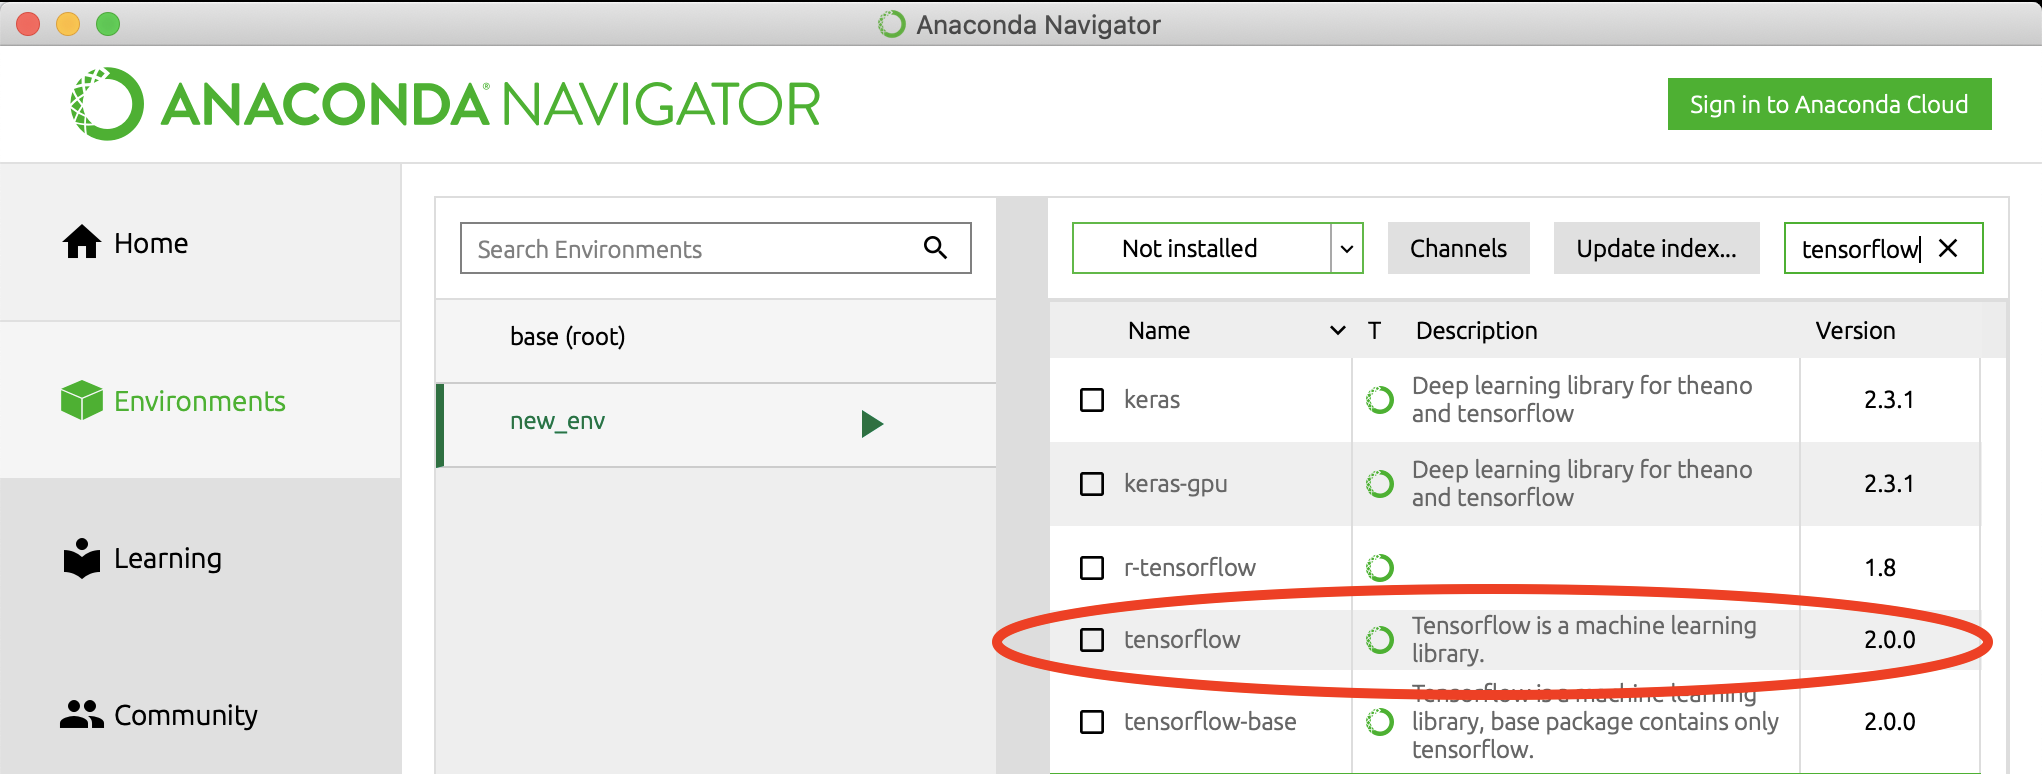
\includegraphics[width=\textwidth]{tensorflow_install.png}
	\end{center}
\begin{itemize}
	\item Installation can be done directly in Anaconda navigator, via \texttt{pip}, or comes pre-installed in Google Collab.
	\item Install \emph{Version 2} so we're all on the same page. 
\end{itemize}
\end{frame}

\begin{frame}
	\frametitle{tensorflow}
	\begin{center}
				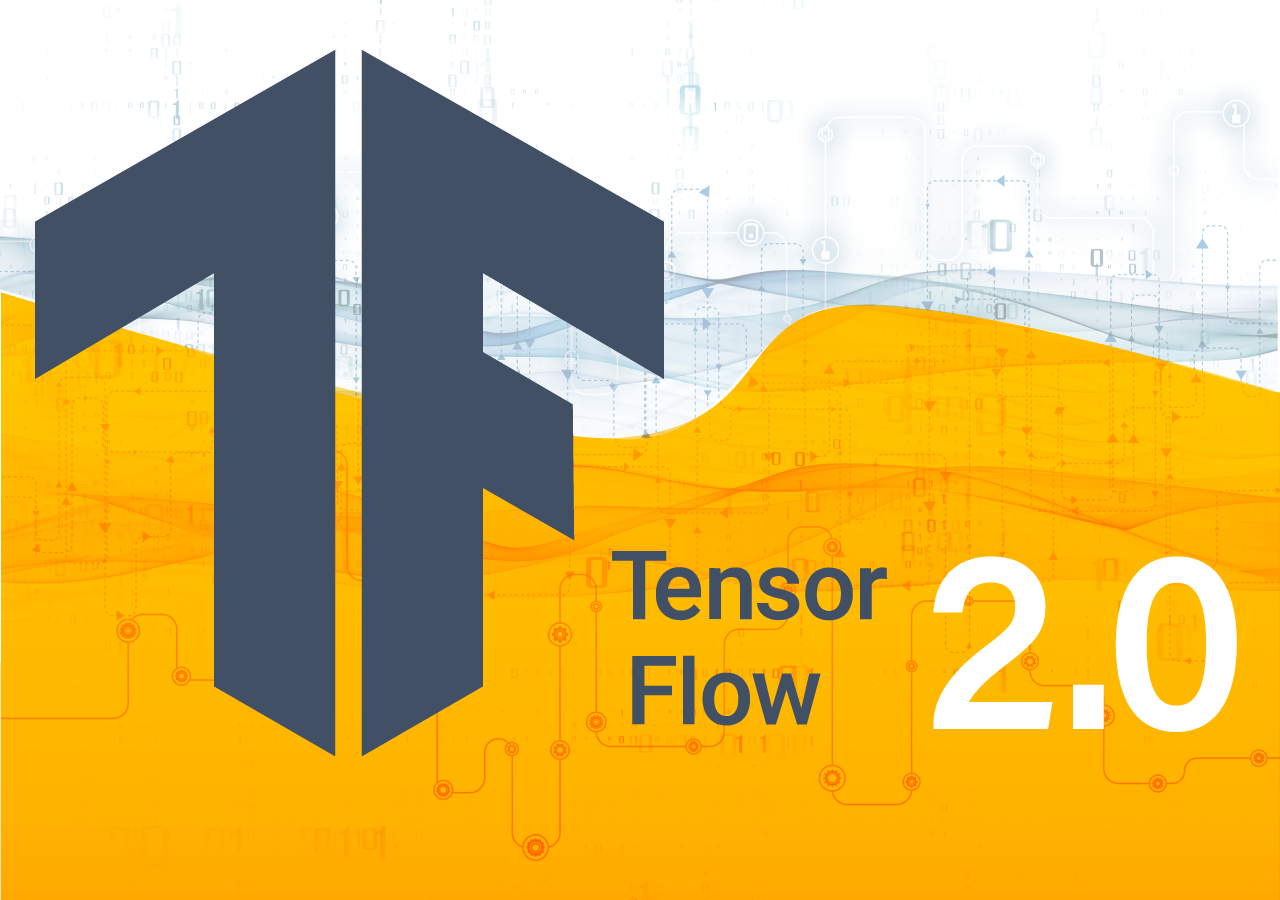
\includegraphics[width=.5\textwidth]{tf2.png}
	\end{center}	
	\texttt{Tensorflow 2} was only released in Fall 2019, so if you are having issues and need Google for answers, make sure to restrict the dates of your search. 
\end{frame}


\begin{frame}
	\frametitle{neural networks}
	\begin{center}
	\alert{\textbf{The} hot-topic in machine learning right now.}
	
	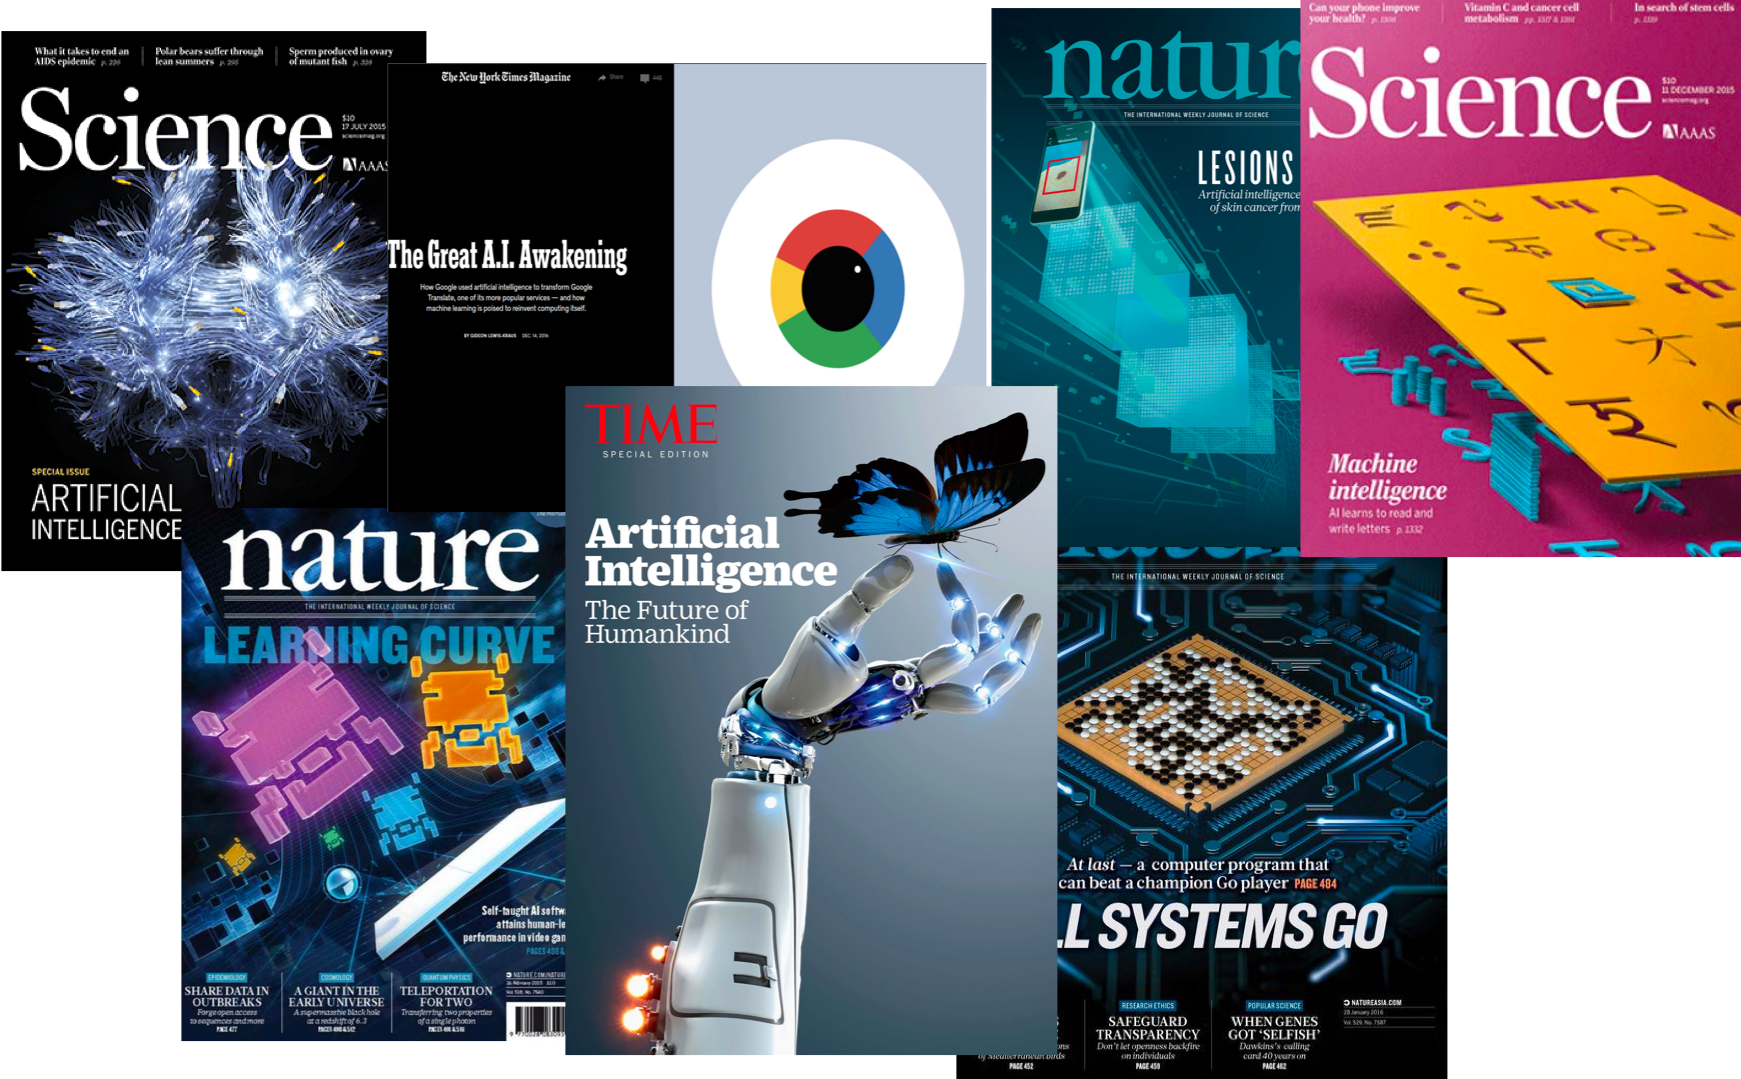
\includegraphics[width=.6\textwidth]{hottopic.png}
	
	Focus of investment at universities, government research labs and funding agencies, and now large tech companies.
	\end{center}

	Studied since the 1940s/50s. \textbf{Why the sudden attention?} More on history of neural networks at the end of lecture. 	
\end{frame}

\begin{frame}
	\frametitle{simple motivating example}
	Classification when data is not linearly separable:
	\begin{center}
		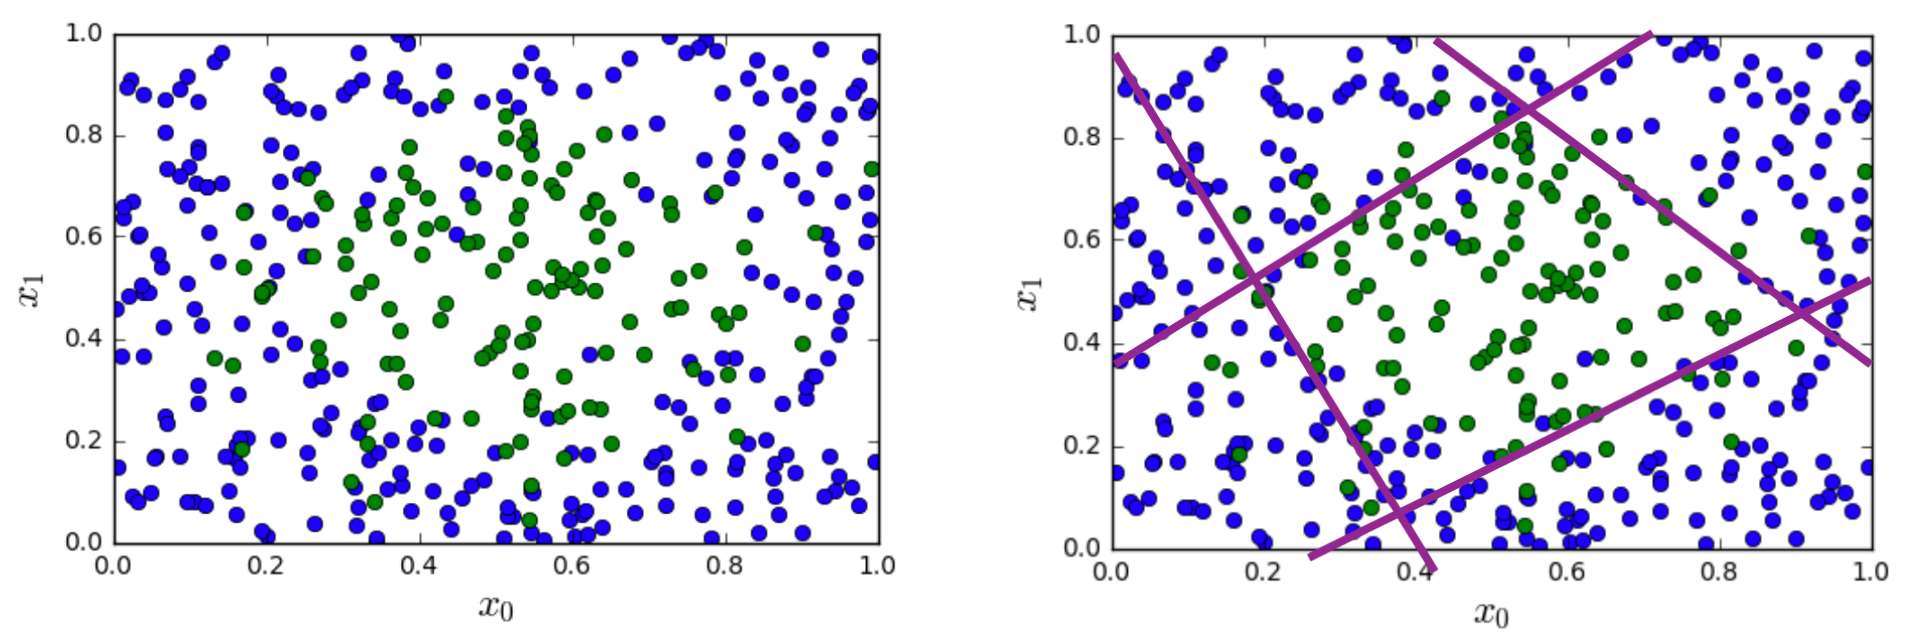
\includegraphics[width=.9\textwidth]{nonsep_chop.png}
	\end{center}
	Could use feature transformations or a non-linear kernel. 
	
	\begin{center}
		\textbf{Alternative approach:} Divide the space up into regions using multiple linear classifiers.
	\end{center}
\end{frame}

\begin{frame}
	\frametitle{simple motivating example}
	For each linear classifier $\vec{\beta}$, add a new $0, 1$ feature for every example $\vec{x} = [x_0,x_1]$ depending on the sign of $\langle \vec{x}, \vec{\beta}\rangle$.
	\vspace{-1em}
	\begin{center}
		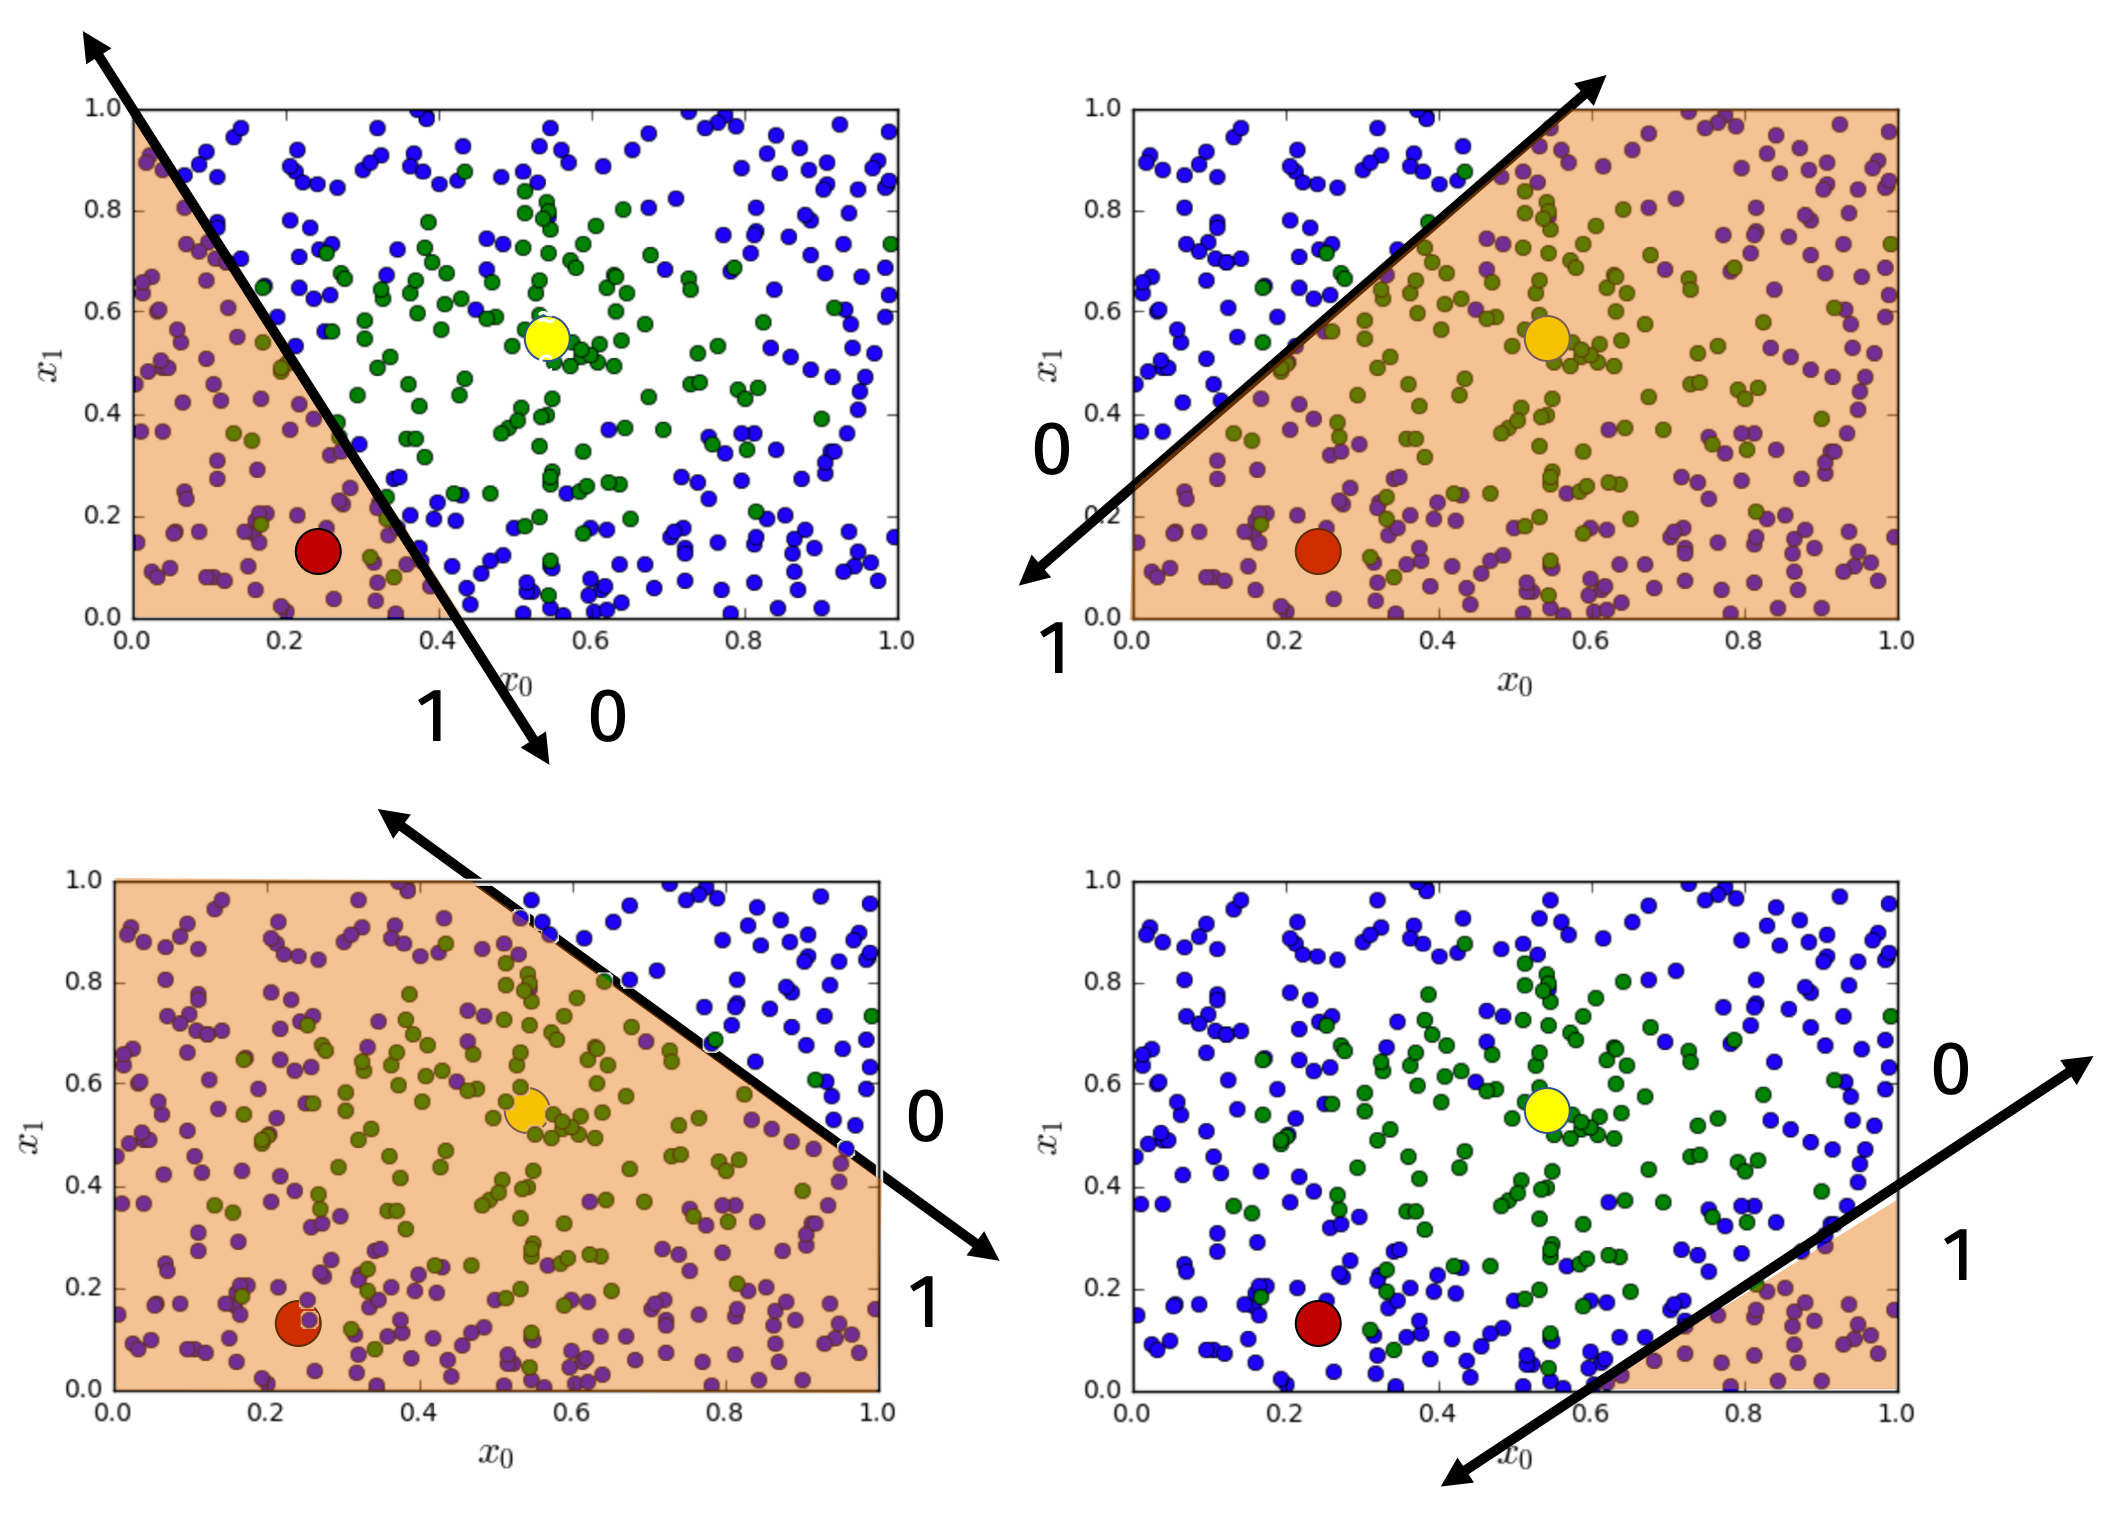
\includegraphics[width=.8\textwidth]{sep_more_formal.png}
	\end{center}
	\vspace{-1em}
	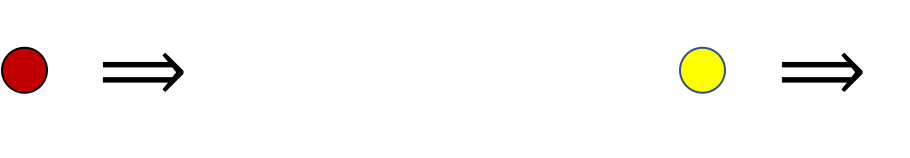
\includegraphics[width=.6\textwidth]{new_features.png}
\end{frame}

\begin{frame}
	\frametitle{simple motivating example}
	\begin{align*}
			\begin{bmatrix}
		.2,.8,\\
		 .5,.5\\ 
		\vdots \\
		.5,1
	\end{bmatrix} 
		\begin{bmatrix}
		\vec{x}_1\\
		\vec{x}_2 \\ 
		\vdots \\
		\vec{x}_n
		\end{bmatrix} \Longrightarrow
		\begin{bmatrix}
		\vec{u}_1\\
		\vec{u}_2 \\ 
		\vdots \\
		\vec{u}_n
		\end{bmatrix}
		= 	\begin{bmatrix}
		0,0,1,0\\
		0,1,1,0\\ 
		\vdots \\
		0,0,0,0
		\end{bmatrix}
	\end{align*}
	\textbf{Question:} After data transformation, how should we map a new vectors $\vec{u}$ to a class label?
		\begin{align*}
	\begin{bmatrix}
		0,0,1,0\\
		0,1,1,0\\ 
		\vdots \\
		0,0,0,0
	\end{bmatrix} \xrightarrow{?}
	\begin{bmatrix}
	0\\
	1 \\ 
	\vdots \\
	0
	\end{bmatrix}
	\end{align*}
\end{frame}

\begin{frame}
	\frametitle{simple motivating example}
	Our machine learning algorithms needs to \textbf{learn two things}:
	\begin{itemize}
		\item The original linear functions which divide our data set into regions (their slopes + intercepts).
		\begin{center}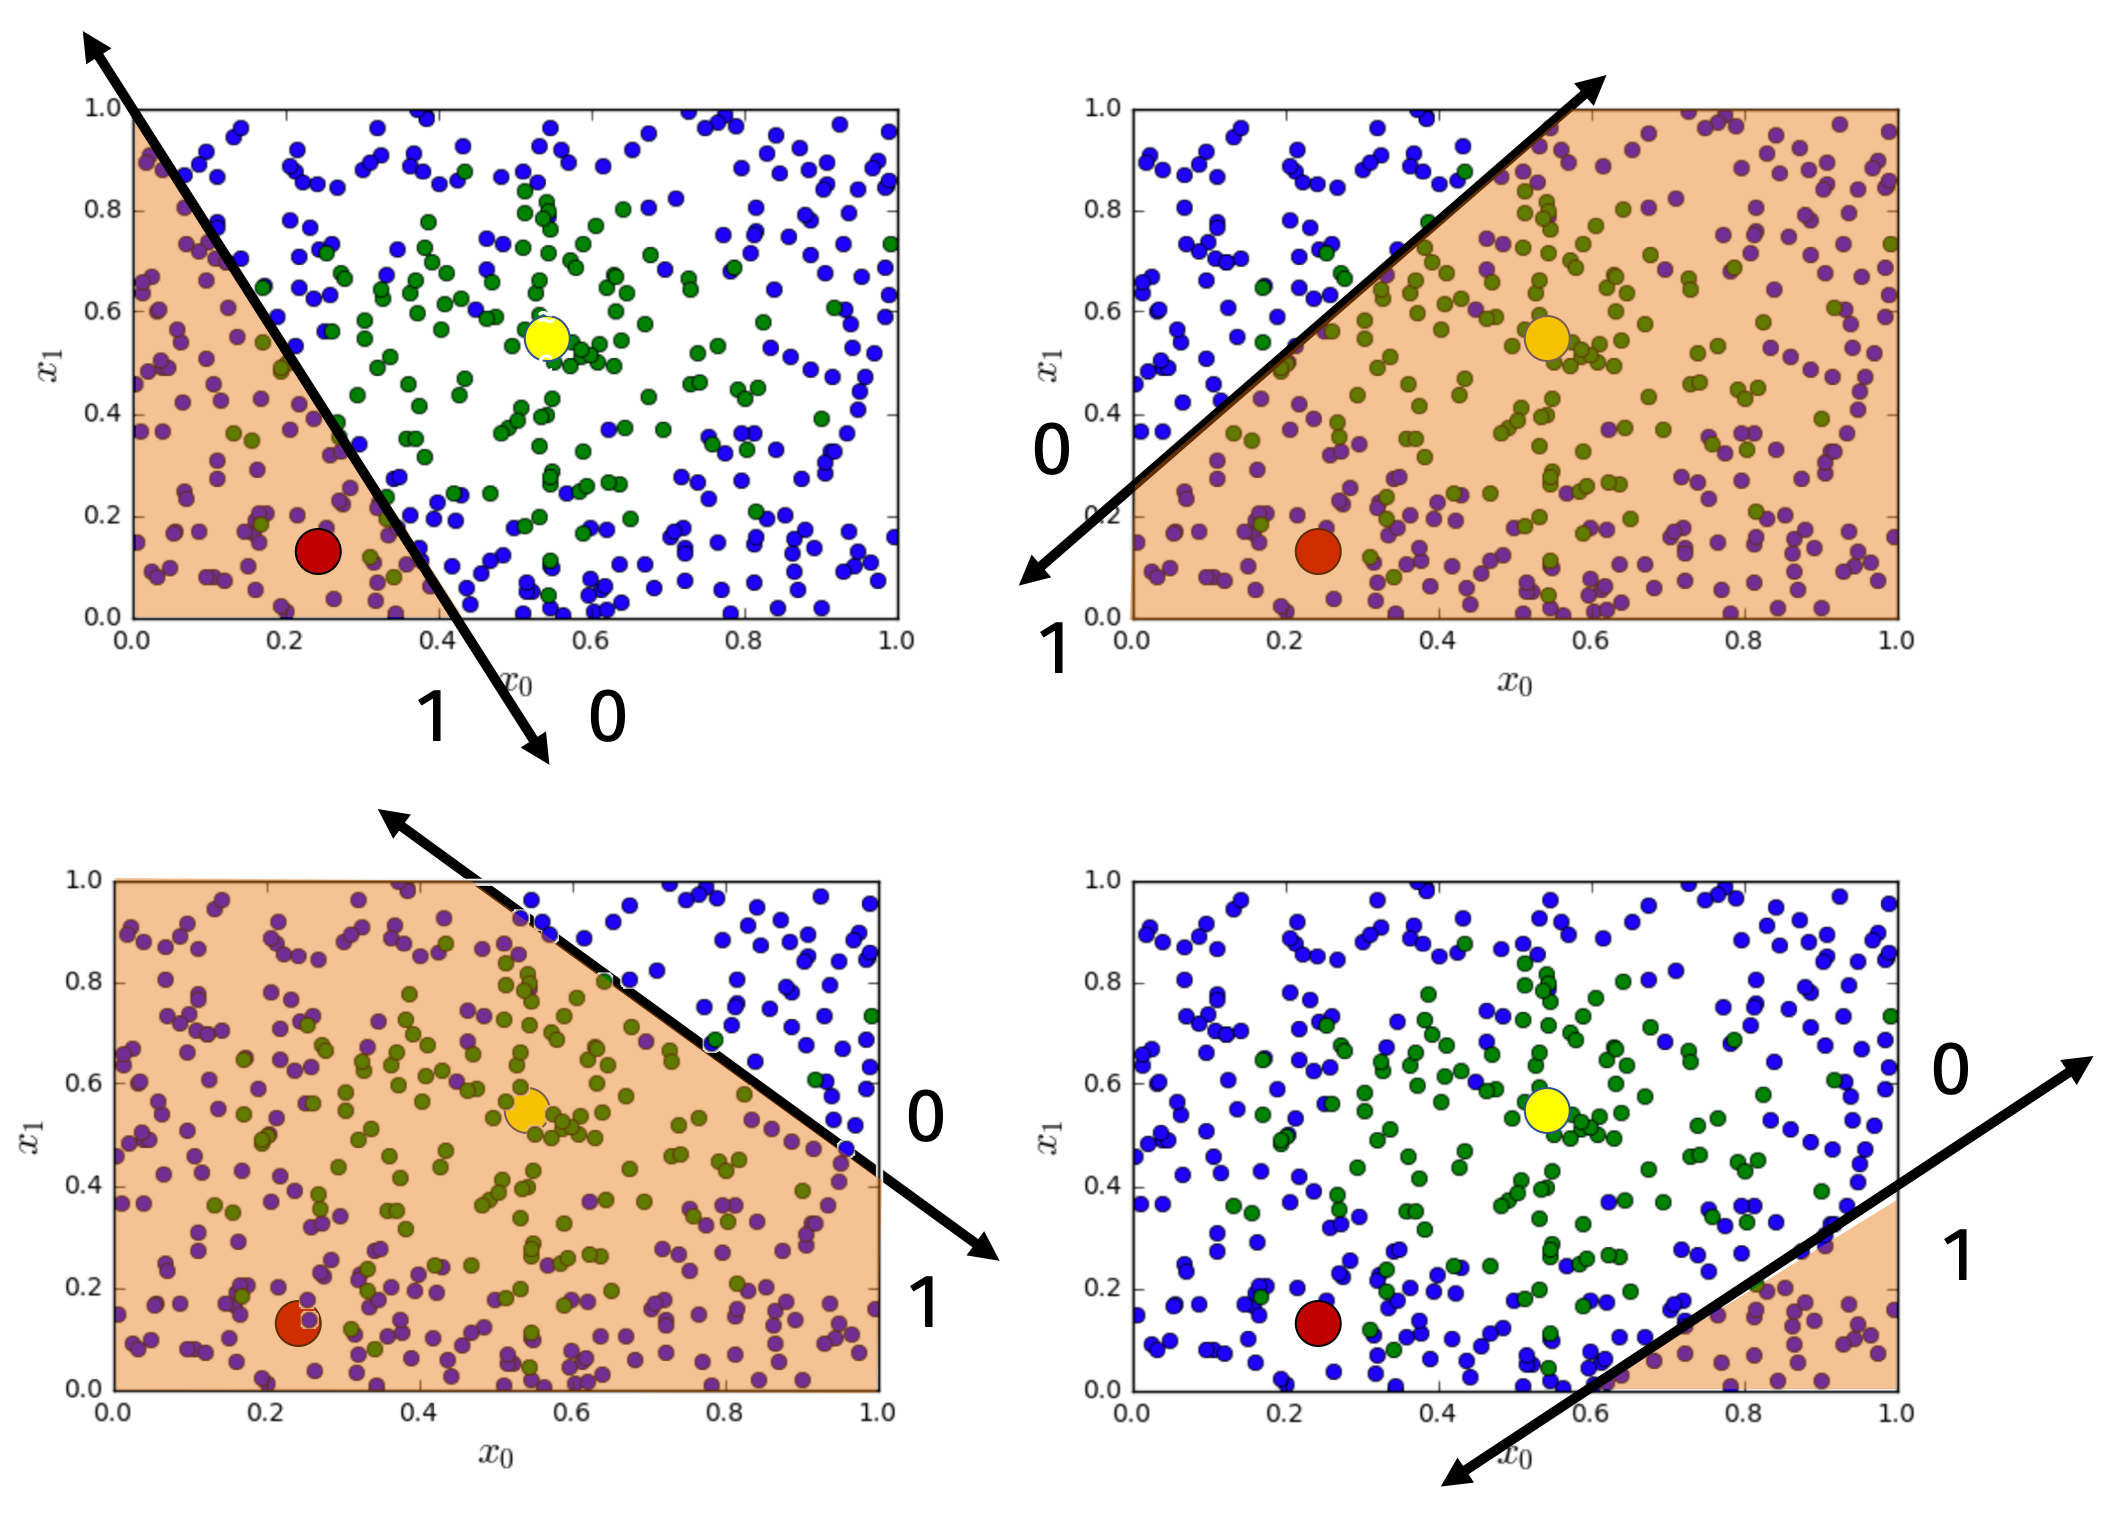
\includegraphics[width=.4\textwidth]{sep_more_formal.png}\end{center}
		\item Another linear function which maps our new features to an output label (typically by thresholding).
	\end{itemize}
	
\end{frame}

\begin{frame}
	\frametitle{possible model}
	\textbf{Input:} $\vec{x} = x_1, \ldots, x_{N_I}$
	
	\textbf{Model:} $f(\vec{x}, \Theta)$:
	\begin{itemize}
		\item $\vec{z}_H\in \R^{N_H} = \bv{W}_H\vec{x} + \vec{b}_h$.
		\item $\vec{u}_H = [\vec{z}_H > 0]$ 
		\item $z_O \in \R = \bv{W}_O\vec{u}_H + b_O$
		\item ${u}_O = [{z}_O > 0]$
	\end{itemize}

	\textbf{Parameters:} $\Theta = [\bv{W}_H\in \R^{N_H\times N_I}, \vec{b}_H\in \R^{N_H} , \bv{W}_O\in \R^{1\times N_H}, {b}_O\in \R]$.
	
	\begin{center}
		$\bv{W}_H$, $\bv{W}_O$ are \emph{weight matrices} and $\vec{b}_H$, ${b}_O$ are \emph{bias} terms that account for the intercepts of our linear functions.  
	\end{center}
\end{frame}

\begin{frame}
	\frametitle{possible model}
	Our model is  function $f$ which makes $\vec{x}$ to a class label $u_O$.\footnote{For {regression}, would cut off at $z_O$ to get continuous output.}

	\begin{center}
		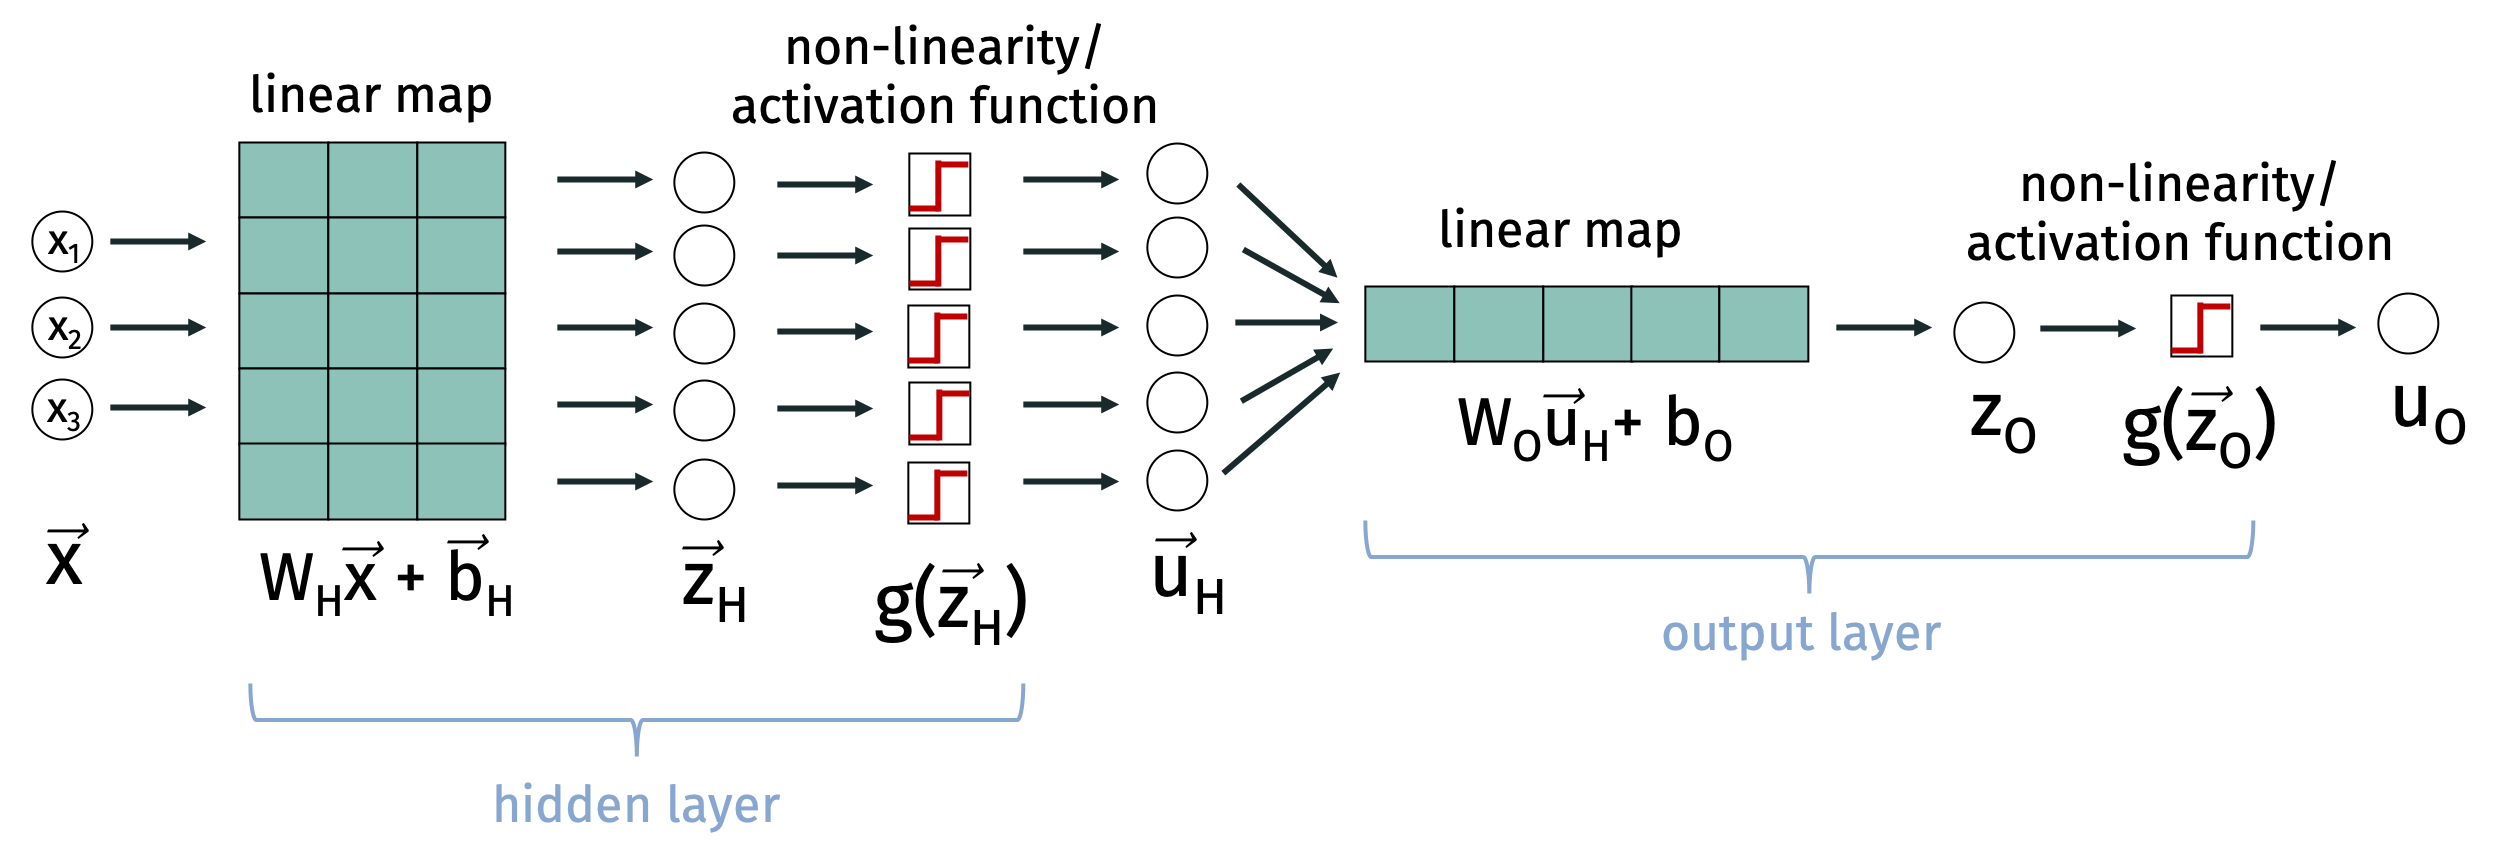
\includegraphics[width=\textwidth]{model_diagram.png}
		
		\vspace{-.5em}
		This is called a ``multilayer perceptron'': one of the oldest types of neural nets. Dates back to Frank Rosenblatt from 1958
	\end{center}	
\vspace{-1em}

\begin{itemize}
	\item Number of input variables $N_I = $
	\item Number of hidden variables $N_H = $
	\item Number of hidden variables $N_O = $
\end{itemize}
	\vspace{.5em}

\end{frame}

\begin{frame}
	\frametitle{possible model}
	Our model is  function $f$ which maps $\vec{x}$ to a class label $u_O$.
	\begin{center}
		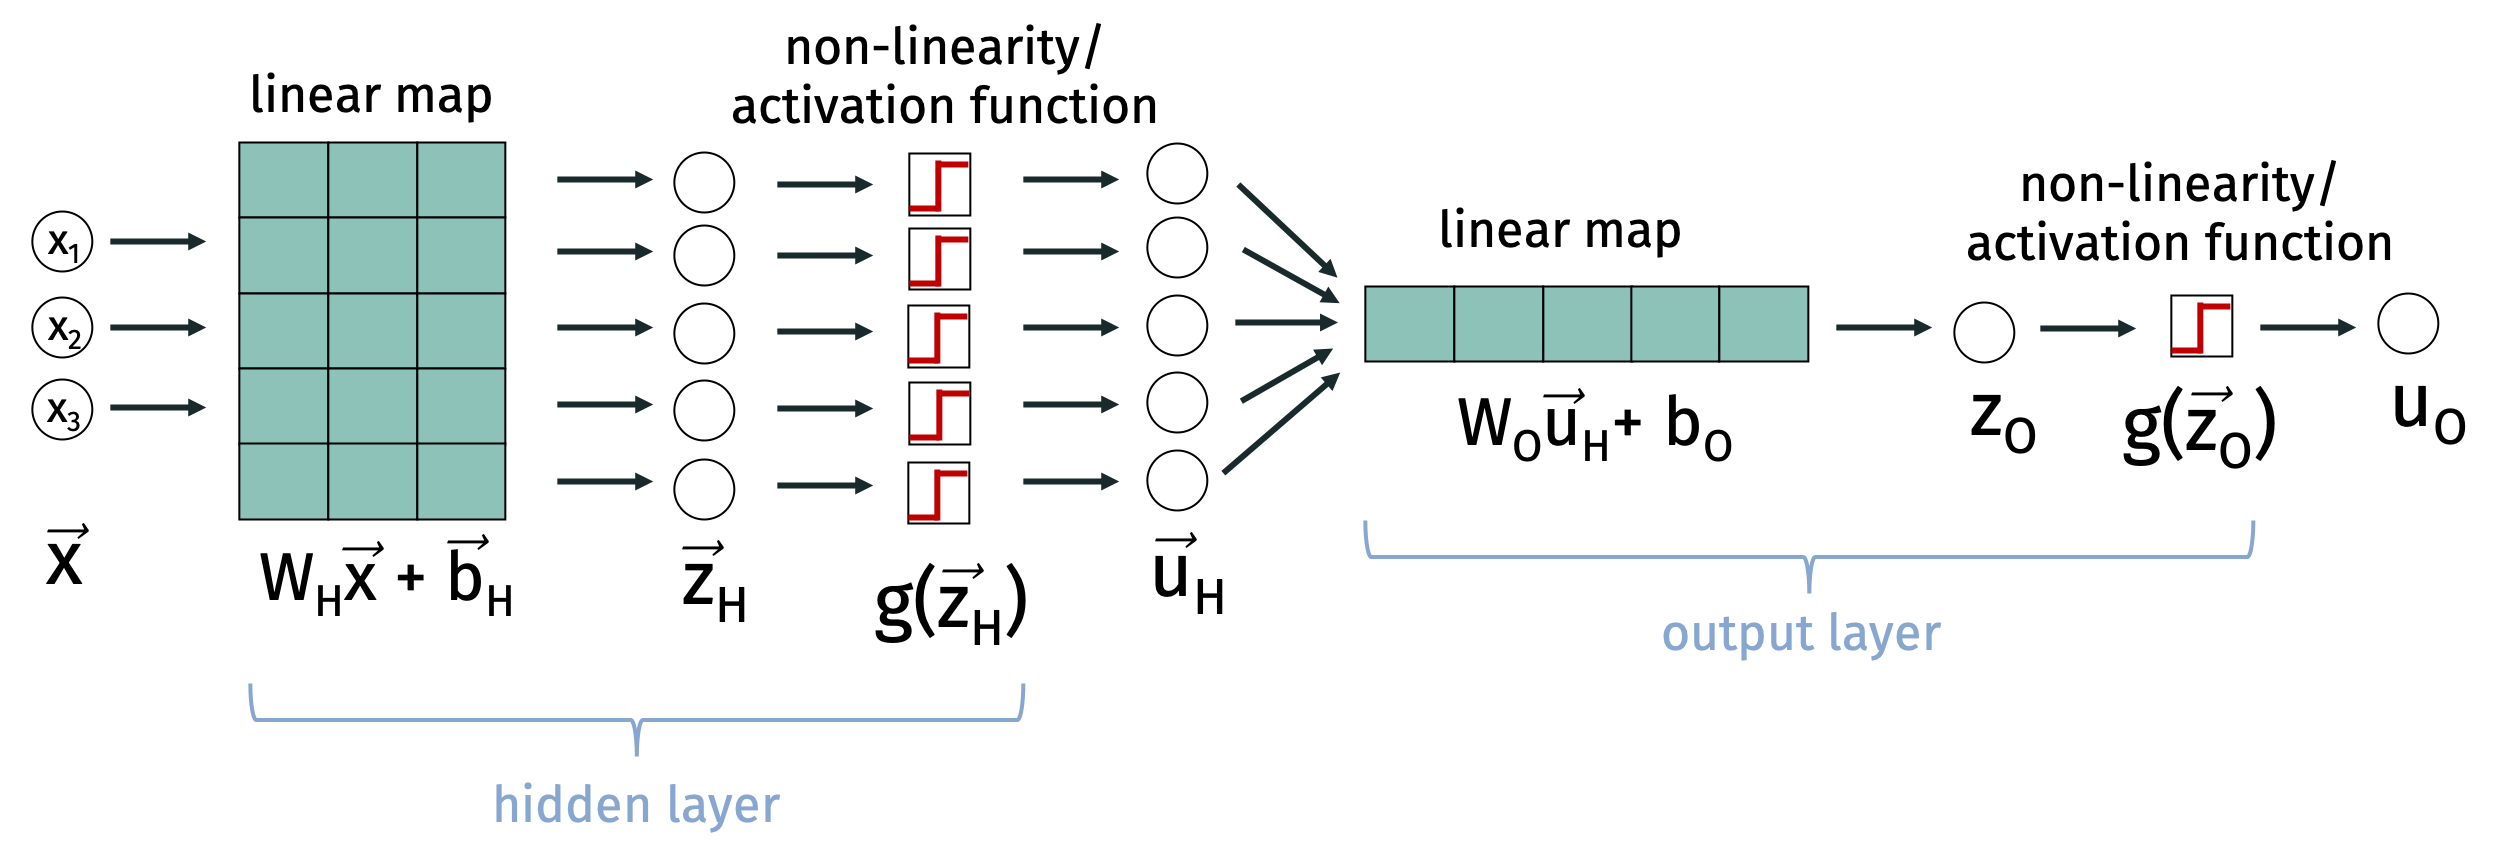
\includegraphics[width=\textwidth]{model_diagram.png}
	\end{center}
	\textbf{Training the model:}
	\begin{itemize}
		\item Choose a loss function $L(f(\vec{x}, \Theta), y)$.
		\item Find optimal parameters: $\Theta^* = \argmin_\Theta \sum_{i=1}^n L(f(\vec{x}_i, \Theta), y_i)$
	\end{itemize}
	\begin{center}
		\alert{\textbf{How to find optimal parameters?}}
	\end{center}
\end{frame}

\begin{frame}
	\frametitle{final model}
	\small
	A more typical model uses smoother \emph{activation functions}, aka \emph{non-linearities}, which are more amenable to computing gradients. E.g. we might use the \textbf{sigmoid function} $g = \frac{1}{1 +e^{-x}}$. 
	\vspace{-1em}
	\begin{center}
		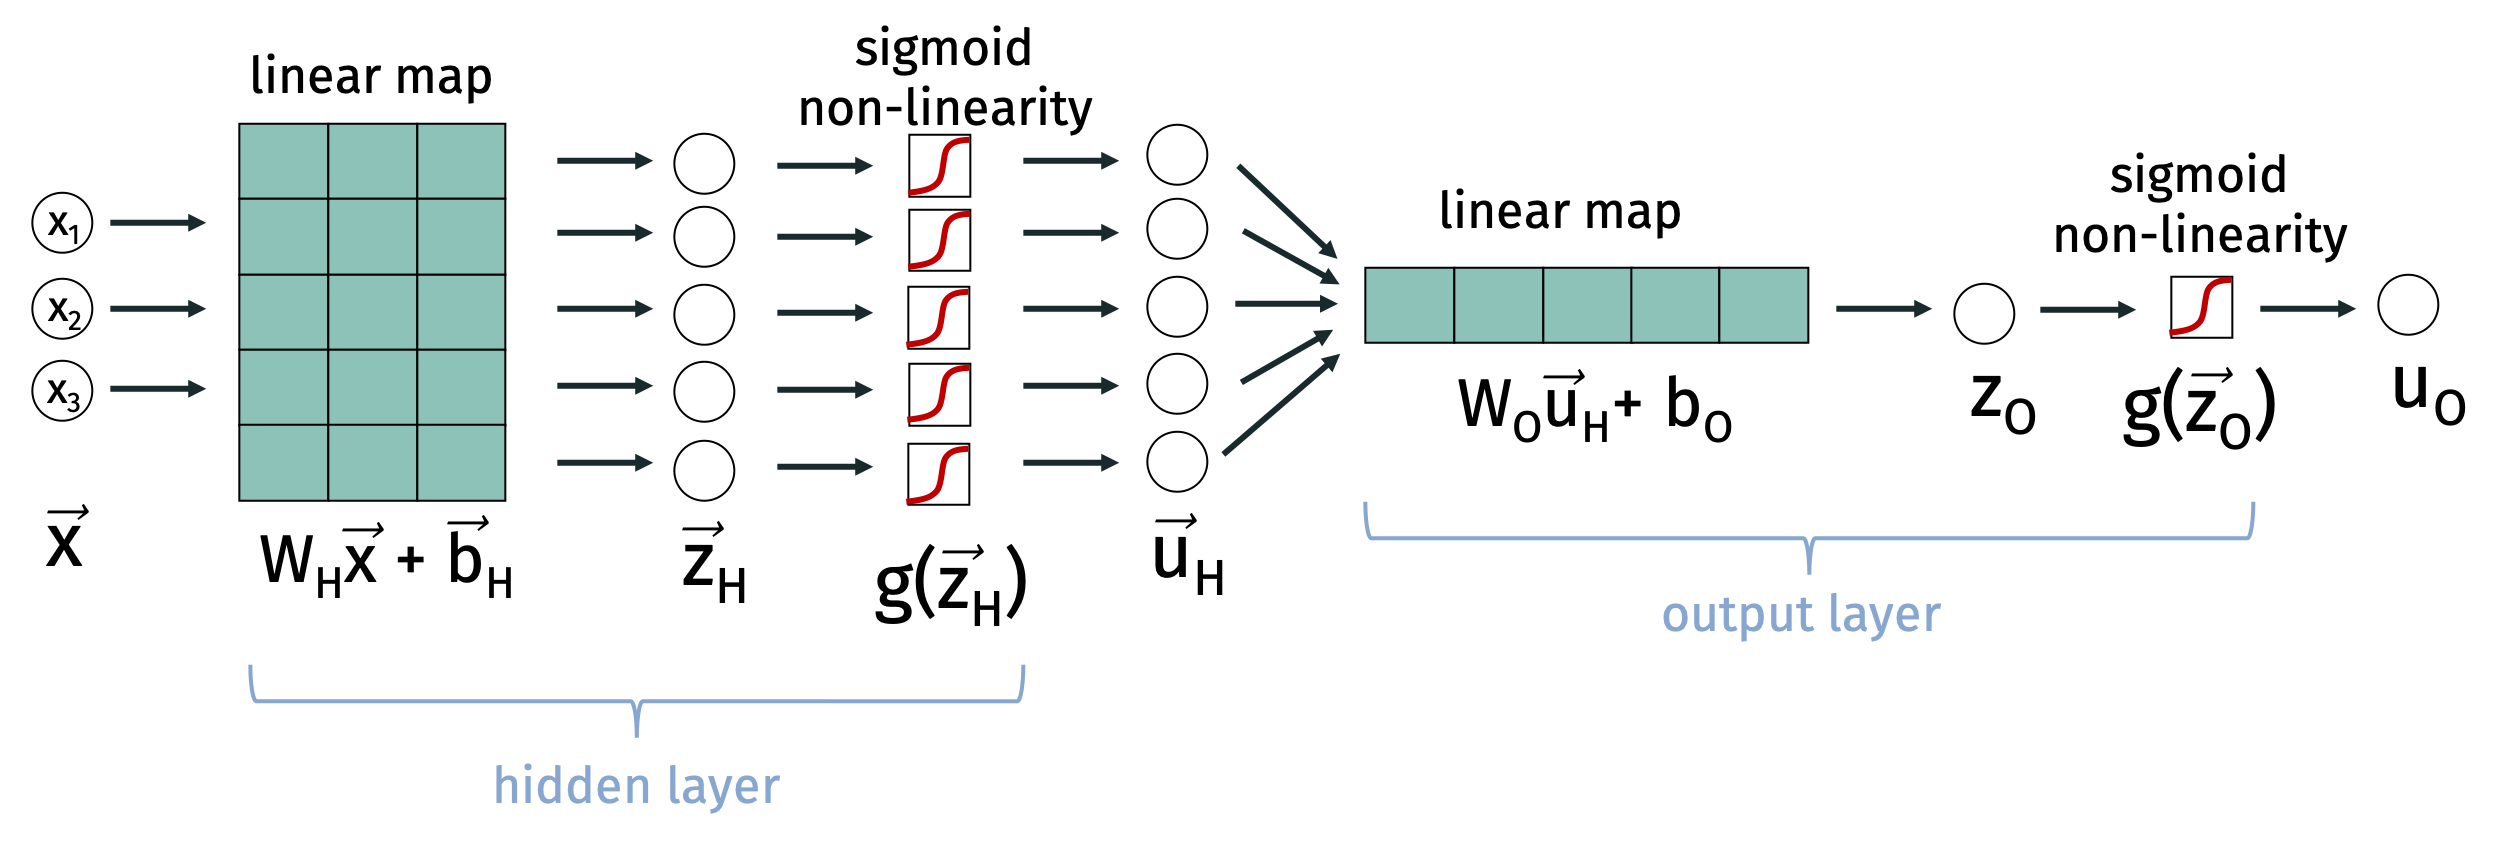
\includegraphics[width=\textwidth]{sigmoid_activation.png}
	\end{center}
\vspace{-2em}
	\begin{itemize}
		\small
		\item Use cross-entropy loss: 
		\begin{align*}
		L(f(\vec{x}_i, \Theta), y) = -y\log(f(\vec{x}_i, \Theta)) - (1-y)\log(1 - f(\vec{x}_i, \Theta))
		\end{align*}
		\item We will discuss later exactly how to compute gradients. 
		\item Will also discuss \emph{categorical cross-entropy/softmax loss} for multi-class problems.
	\end{itemize}
\end{frame}

\begin{frame}
	\frametitle{final model}
	Intuitively switching to a sigmoid activation is not that different from using the step function.\footnote{Sometimes called the ``Heaviside step function'' in machine learning.}
	\begin{center}
		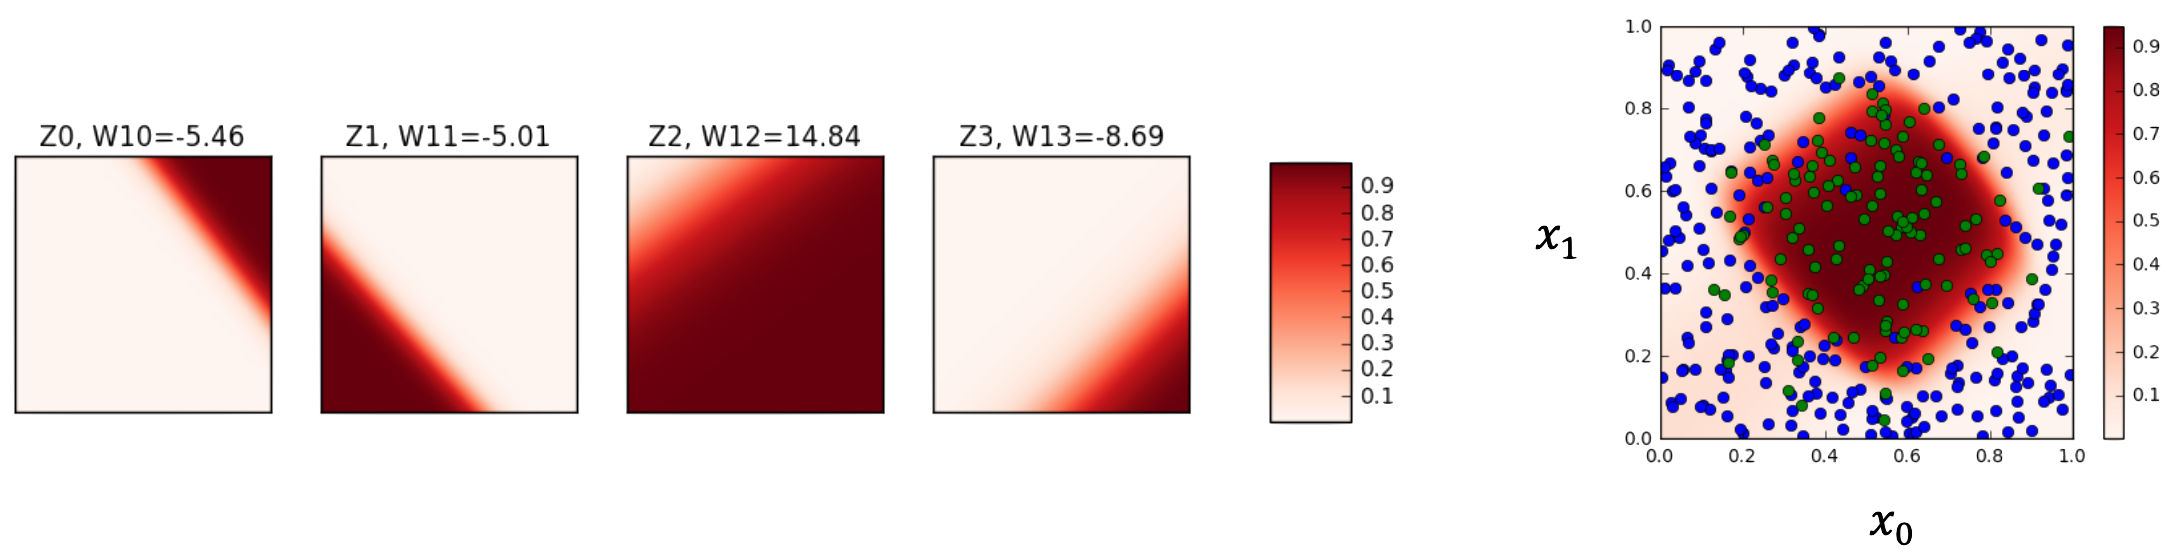
\includegraphics[width=\textwidth]{soft_class.png}
	\end{center}
\end{frame}

\begin{frame}
	\frametitle{hyperparameters}
	\textbf{Things we can change in this basic classification network:}
	\begin{itemize}
		\item More or less hidden variables.
		\item We could add more layers.
		\item Different non-linearity/activation function.
		\item Different loss function (more on that next class). 
	\end{itemize}
	\begin{center}
		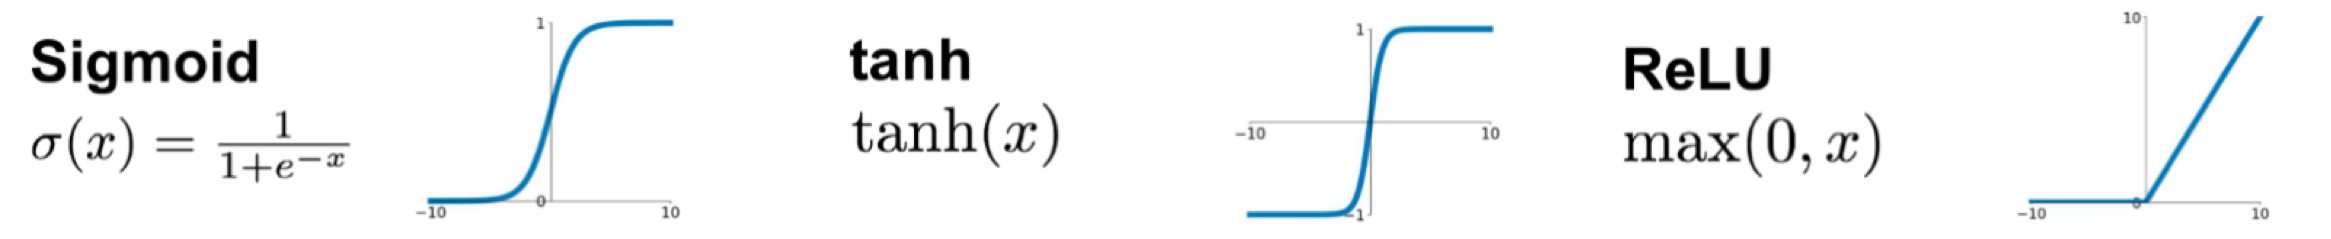
\includegraphics[width=\textwidth]{activation_functions.png}
	\end{center}
\end{frame}

\begin{frame}
	\frametitle{test your intuition}
	\textbf{How many hidden variables (e.g. splitting hyperplanes) would be needed to classify this dataset correctly?}
	\begin{center}
		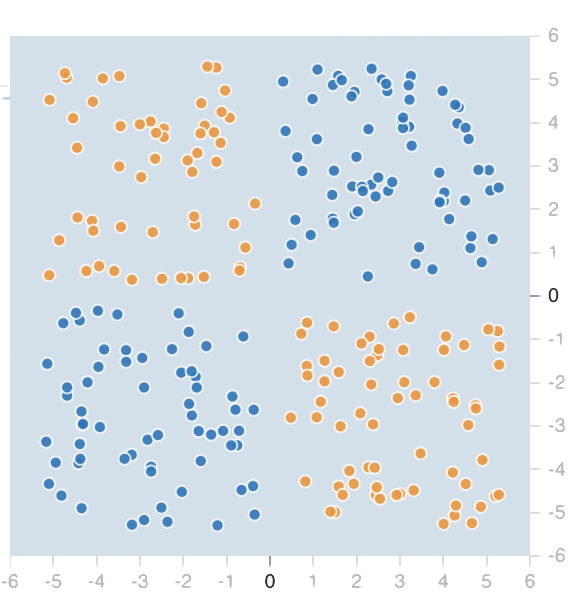
\includegraphics[width=.4\textwidth]{playground_example.png}
		
		\url{https://playground.tensorflow.org/}
	\end{center}
\end{frame}

\begin{frame}[t]
	\frametitle{test your intuition}
		\begin{center}
		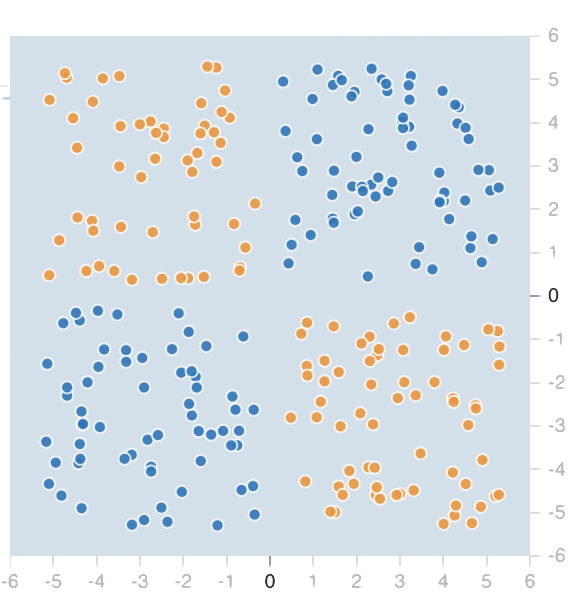
\includegraphics[width=.3\textwidth]{playground_example.png}
	\end{center}
	
\end{frame}

\begin{frame}
	\frametitle{notation}
	\textbf{Another common diagram for a 2-layered network:}
	\begin{center}
		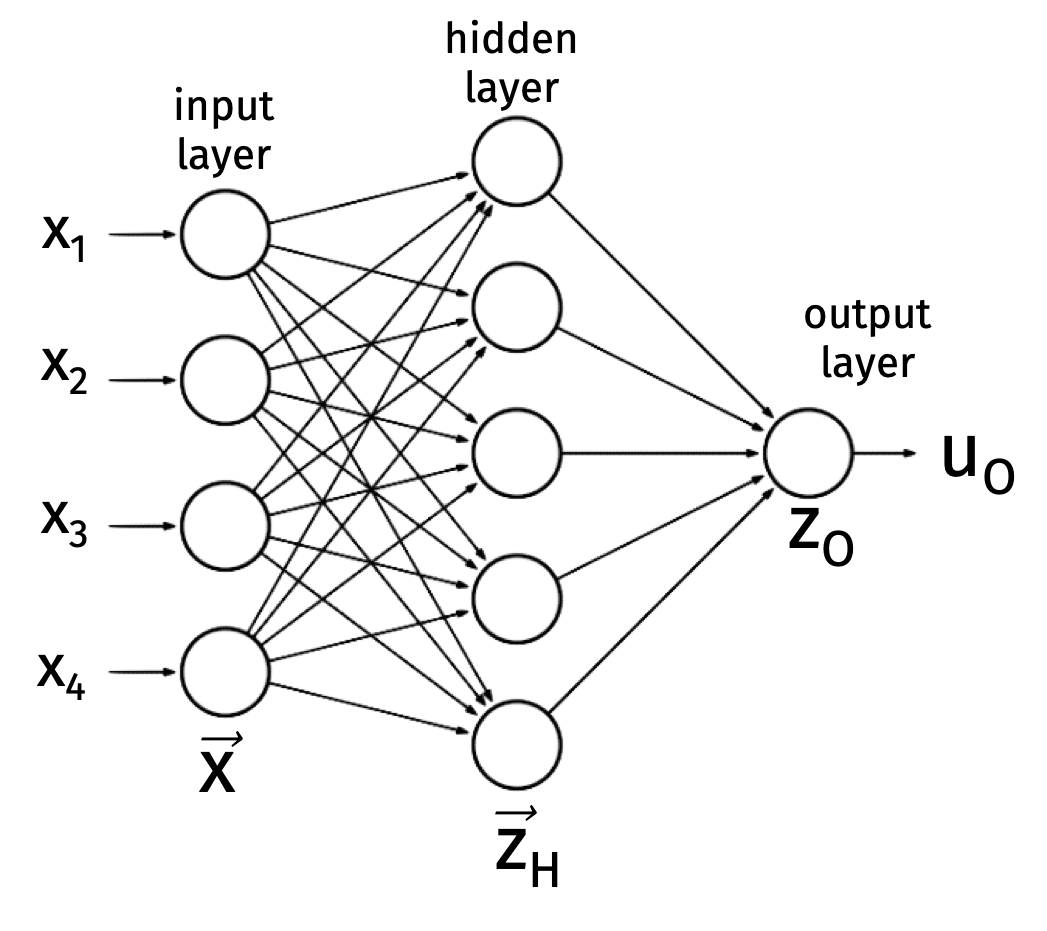
\includegraphics[width=.6\textwidth]{noweights.png}
	\end{center}
\end{frame}

\begin{frame}
	\frametitle{notation}
	\textbf{Neural network math:}
	\begin{center}
		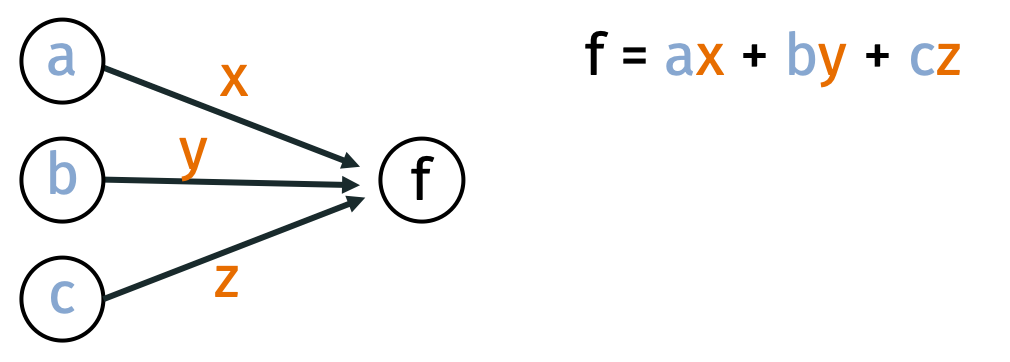
\includegraphics[width=.6\textwidth]{neural_math.png}
	\end{center}
\end{frame}

\begin{frame}
	\frametitle{notation}
	\textbf{How to interpret:}
	\vspace{-1em}
	\begin{center}
		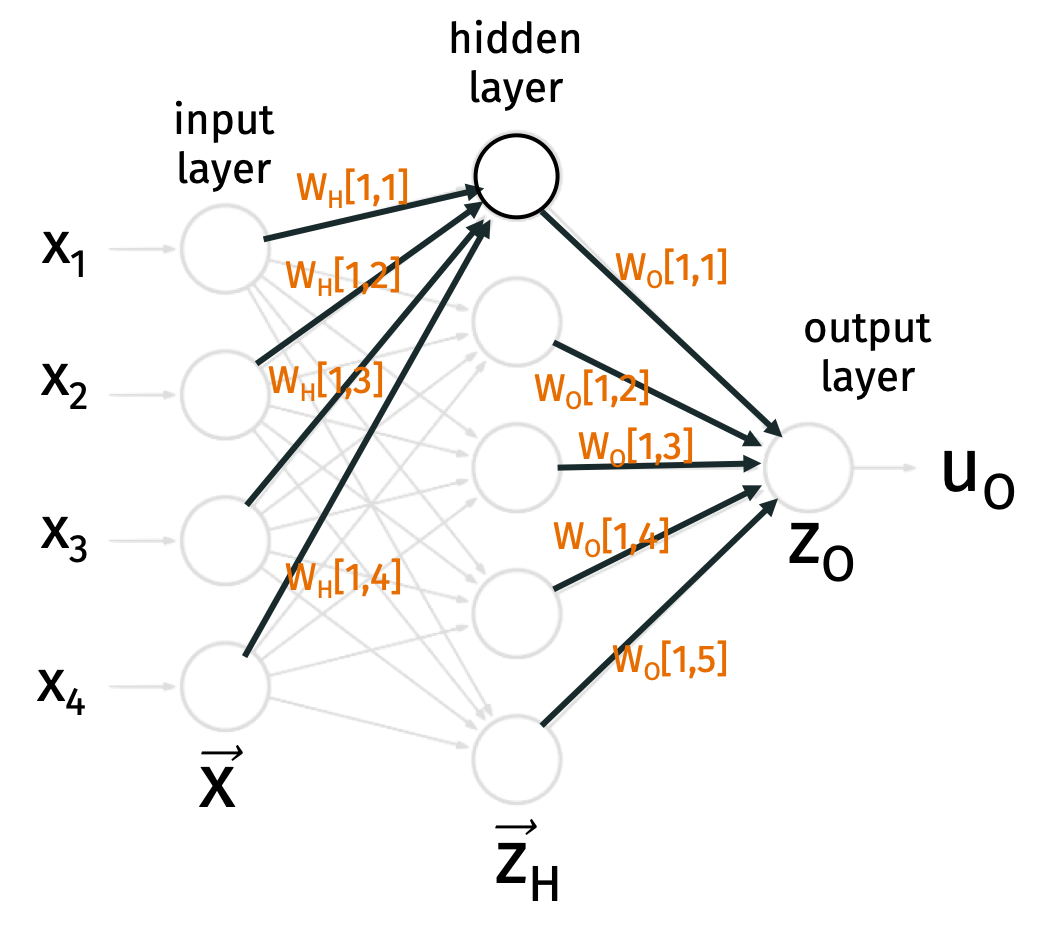
\includegraphics[width=.6\textwidth]{weights1.png}
	\end{center}
\vspace{-1.5em}
$\bv{W}_H$ and $\bv{W}_O$ are our weight matrices from before. 

\textbf{Note:} This diagram does not explicitly show the bias terms or the non-linearity. 
\end{frame}

\begin{frame}
	\frametitle{notation}
	\textbf{How to interpret:}
	\vspace{-1em}
	\begin{center}
		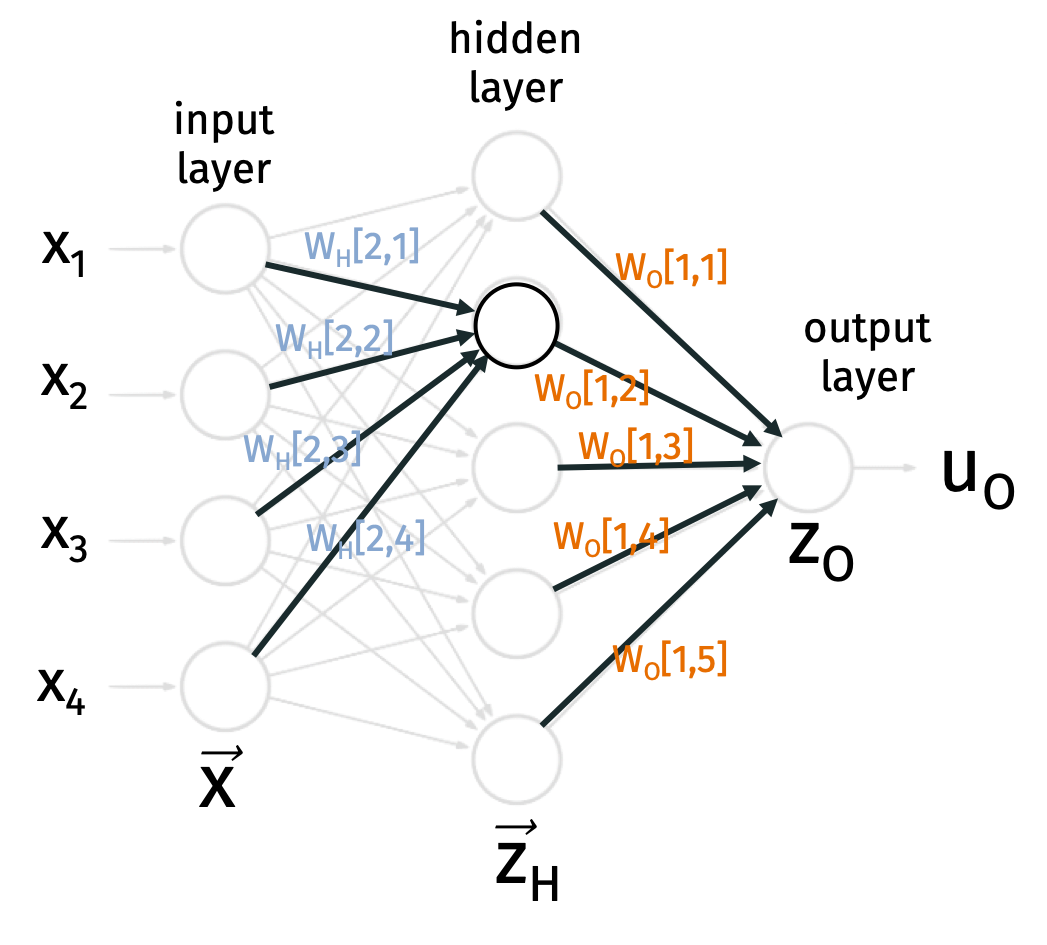
\includegraphics[width=.6\textwidth]{weights2.png}
	\end{center}
\vspace{-1.5em}
$\bv{W}_H$ and $\bv{W}_O$ are our weight matrices from before. 

\textbf{Note:} This diagram depicts a network with \textbf{``fully-connected''} layers.
\end{frame}

\begin{frame}
	\frametitle{connection to biology}
	\small
	\textbf{Simplified model of the brain:}
	\begin{columns}
		\begin{column}{.55\textwidth}
			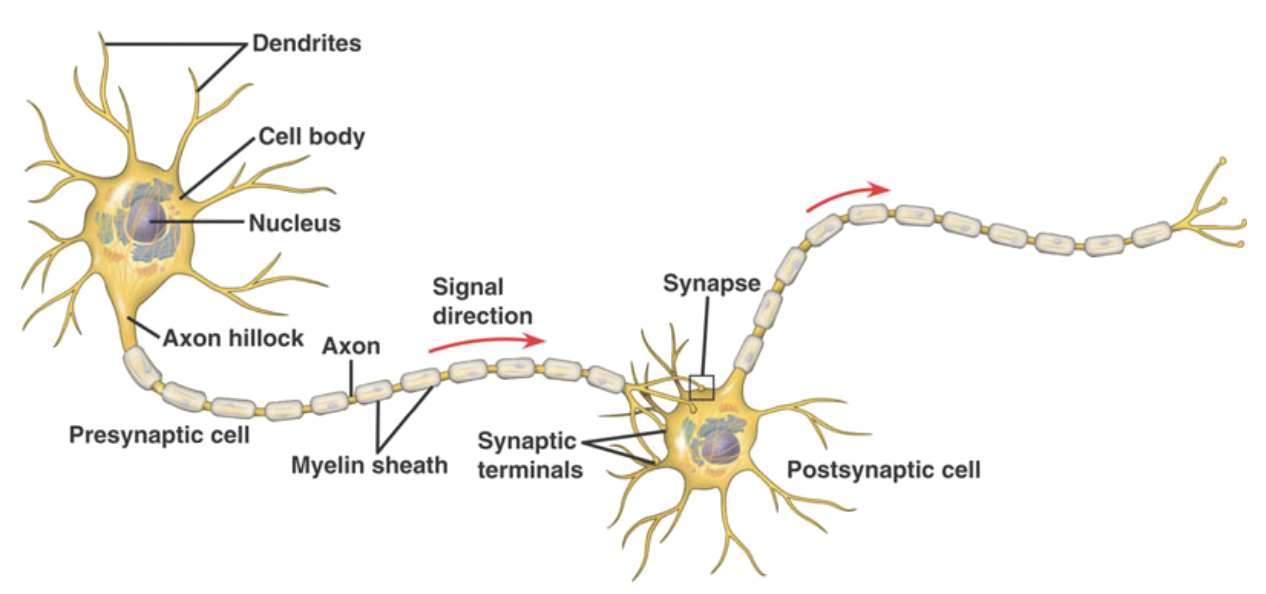
\includegraphics[width=\textwidth]{neurons.png}
		\end{column}
		\begin{column}{.45\textwidth}
			\textbf{Dendrites}: Input electrical current from other neurons.
			
			\textbf{Axon}: Output electrical current to other neurons.
			
			\textbf{Synapse}: Where these two connect.
		\end{column}
	\end{columns}
	A neuron ``fires'' (outputs a non-zero electric charge) if it receives enough cumulative electrical input from the neurons connected to it. 
	\begin{center}
		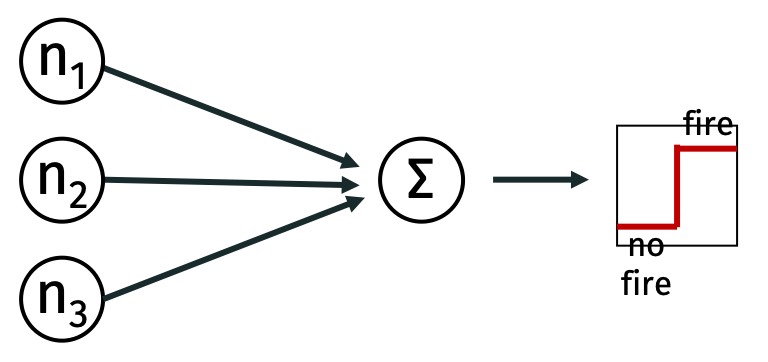
\includegraphics[width=.4\textwidth]{neural_model.png}
	\end{center}
	Output charge can be positive \emph{or} negative (excitatory vs. inhibitory). 
\end{frame}

\begin{frame}
	\frametitle{connection to biology}
	\textbf{Inspired early work on neural networks:}
	\begin{itemize}
		\item 1940s Donald Hebb proposed a Hebbian learning rule for how brains neurons change over time to allow learning.
		\item 1950s Frank Rosenblatt's Perceptron is one of the first ``artifical'' neural networks.
		\item Continued work throughout the 1960s. 
	\end{itemize}
\textbf{Main issue with neural network methods:} They are \emph{hard to train}. Generally require a lot of computation power. Also pretty finicky: user needs to be careful with initialization, regularization, etc. when training.  Often requires a lot of experimentation to get right.
\end{frame}

\begin{frame}
	\frametitle{early neural network explosion}
	Around 1985 a few groups (re)-discovered the \textbf{backpropagation algorithm} which allows for efficient training of neural nets via \textbf{gradient descent}. Along with increased computational power this lead to a resurgence of interest in neural network models. 
	\begin{center}		
		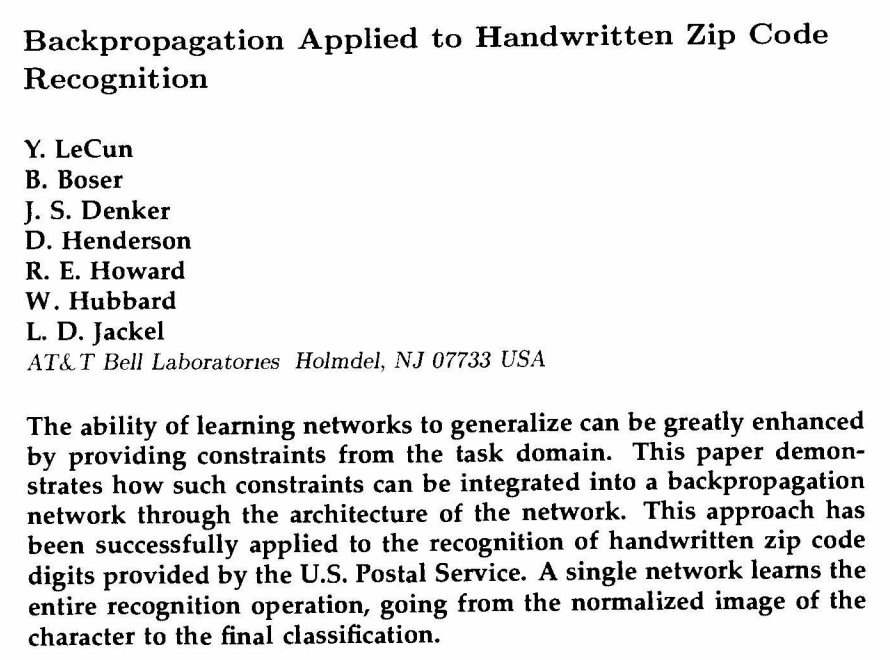
\includegraphics[width=.5\textwidth]{mnistbackprop.png}
	\end{center}
Good performance on problems like digit recognition.
\end{frame}

\begin{frame}
	\frametitle{neural network decline}
	In the 1990s and early 2000s, kernel methods, SVMs, and probabilistic methods began to dominate the literature in machine learning:
	\begin{itemize}
		\item Work well ``out of the box".
		\item Relatively easy to understand theoretically.
		\item Not too computationally expensive for moderately sized datasets. 
	\end{itemize}
\textbf{Fun blog post to check out from 2005:} \url{http://yaroslavvb.blogspot.com/2005/12/trends-in-machine-learning-according.html}
\end{frame}

\begin{frame}
	\frametitle{neural network decline}
		\footnotesize
	Finding trends in machine learning by search papers in Google Scholar that match a certain keyword:
	\begin{center}		
		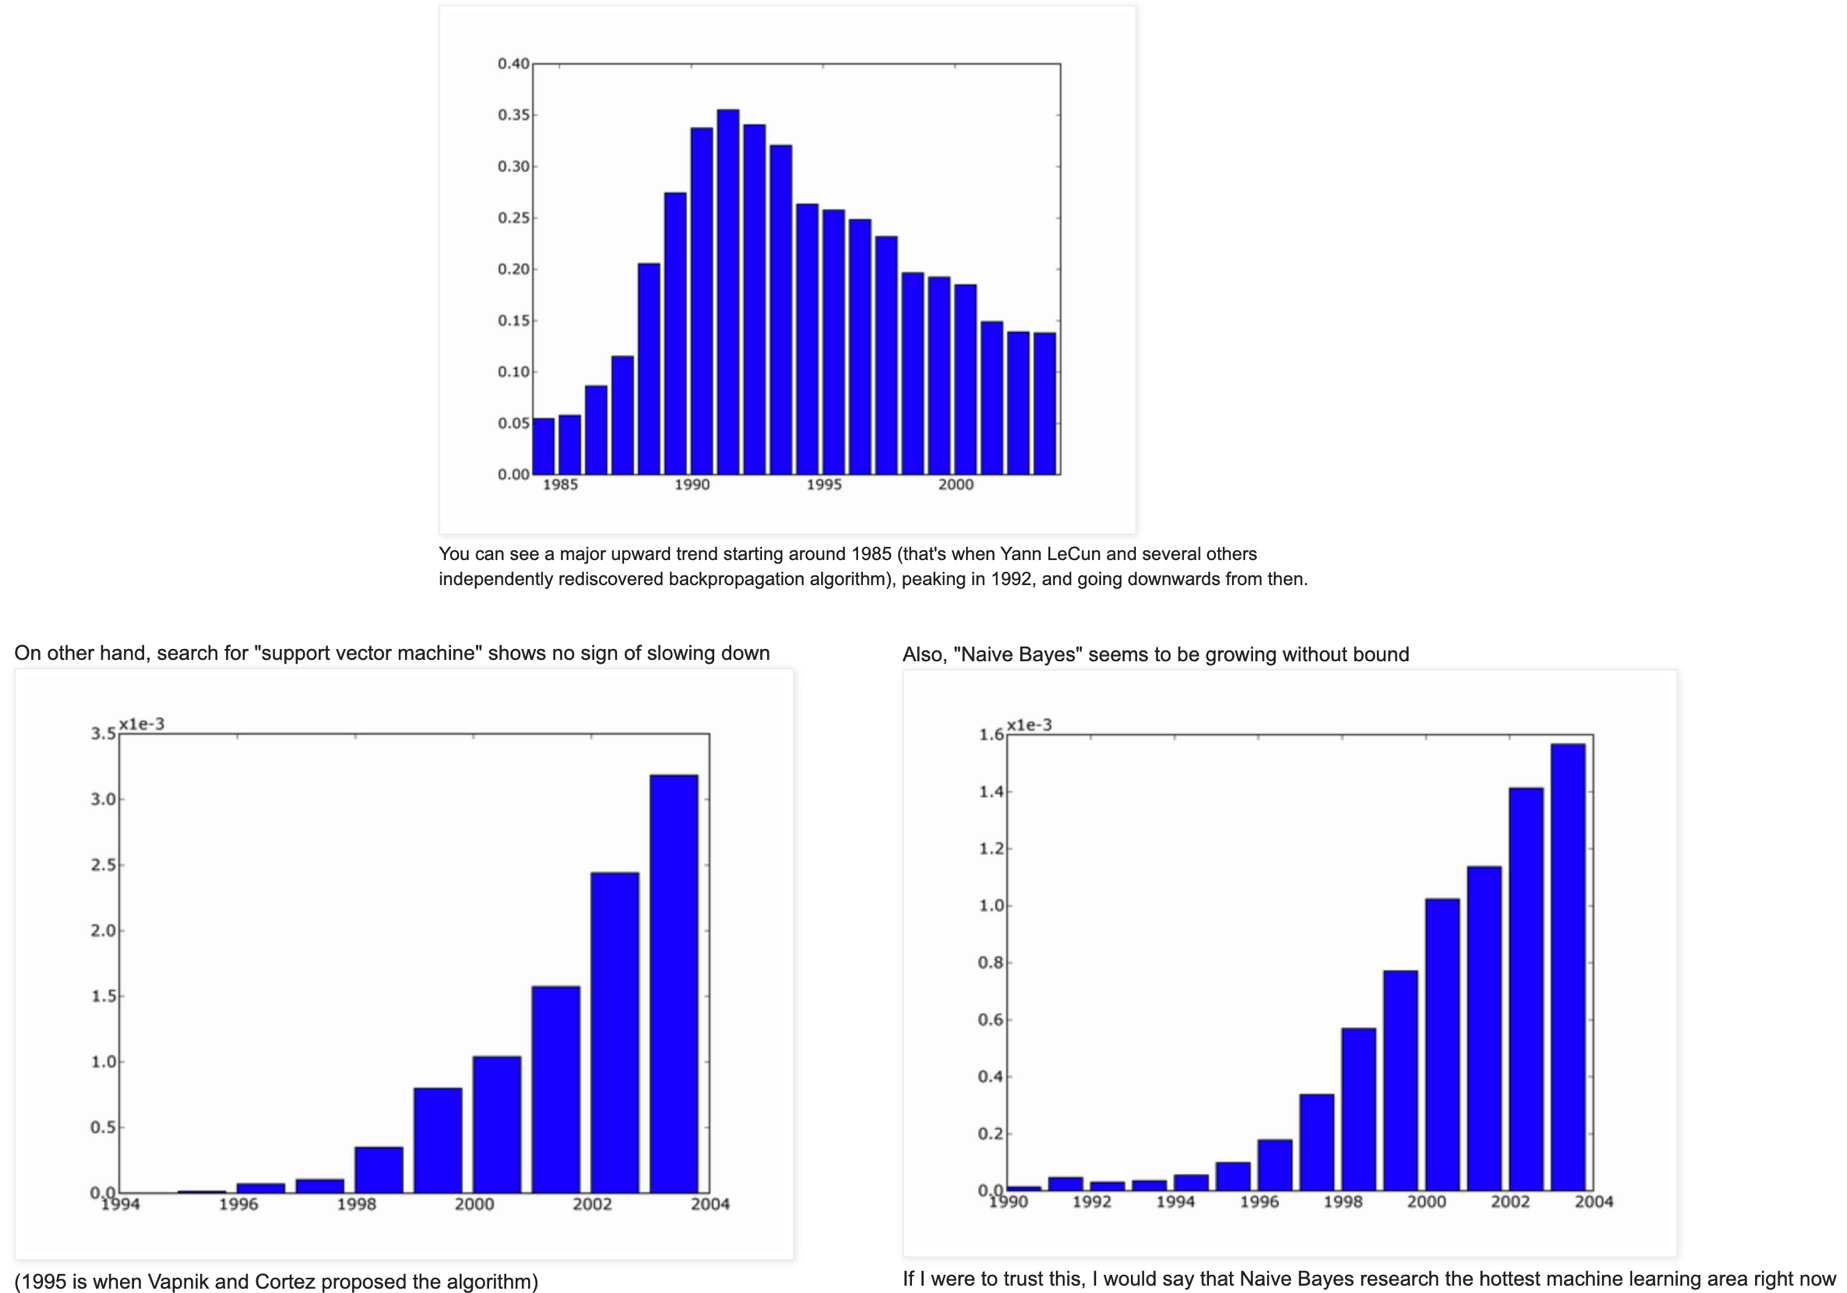
\includegraphics[width=.9\textwidth]{trends.png}
	\end{center}
\end{frame}

\begin{frame}
	\frametitle{modern neural networks}
	\begin{center}
		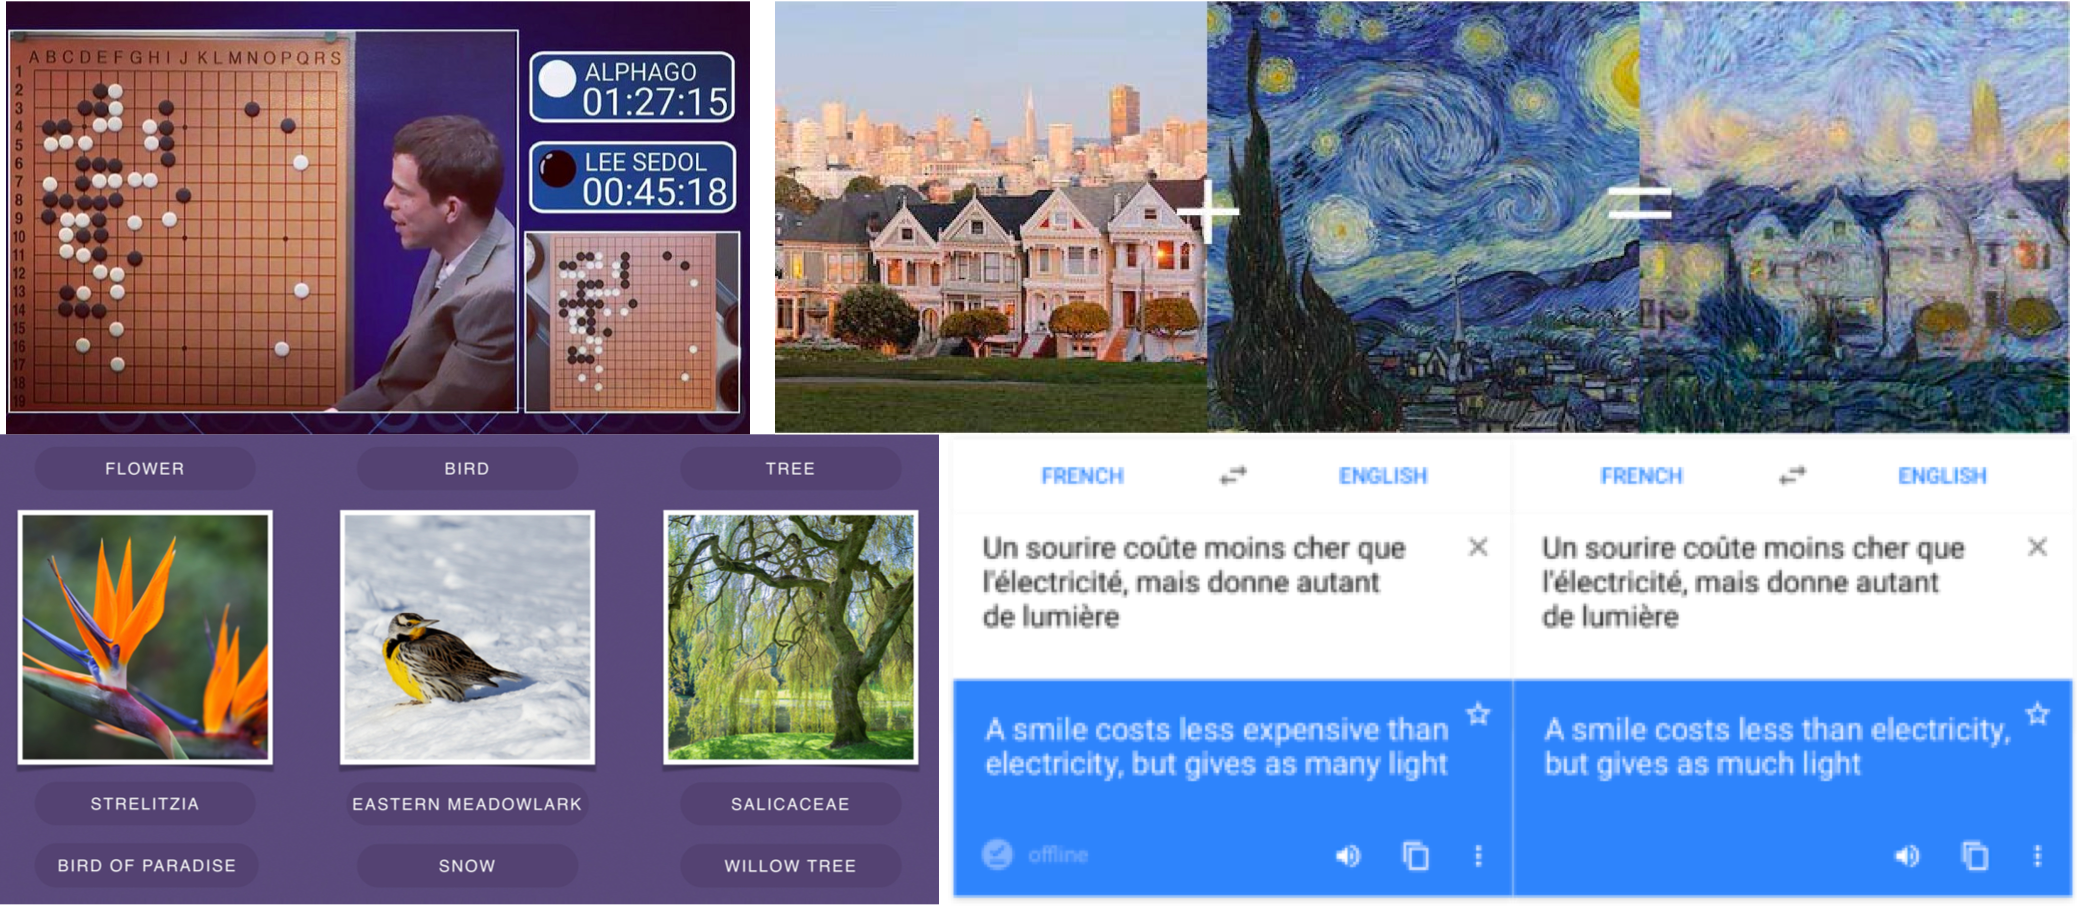
\includegraphics[width=.8\textwidth]{newstuff.png}
	\end{center}
Recent state-of-the-art results in \emph{game playing}, \emph{image recognition}, \emph{content generation}, \emph{natural language processing}, \emph{machine translation}, many other areas.  
\end{frame}

\begin{frame}
	\frametitle{modern neural networks}
	All changed with the introduction of AlexNet and the 2012 ImageNet Challenge...
	\begin{center}
		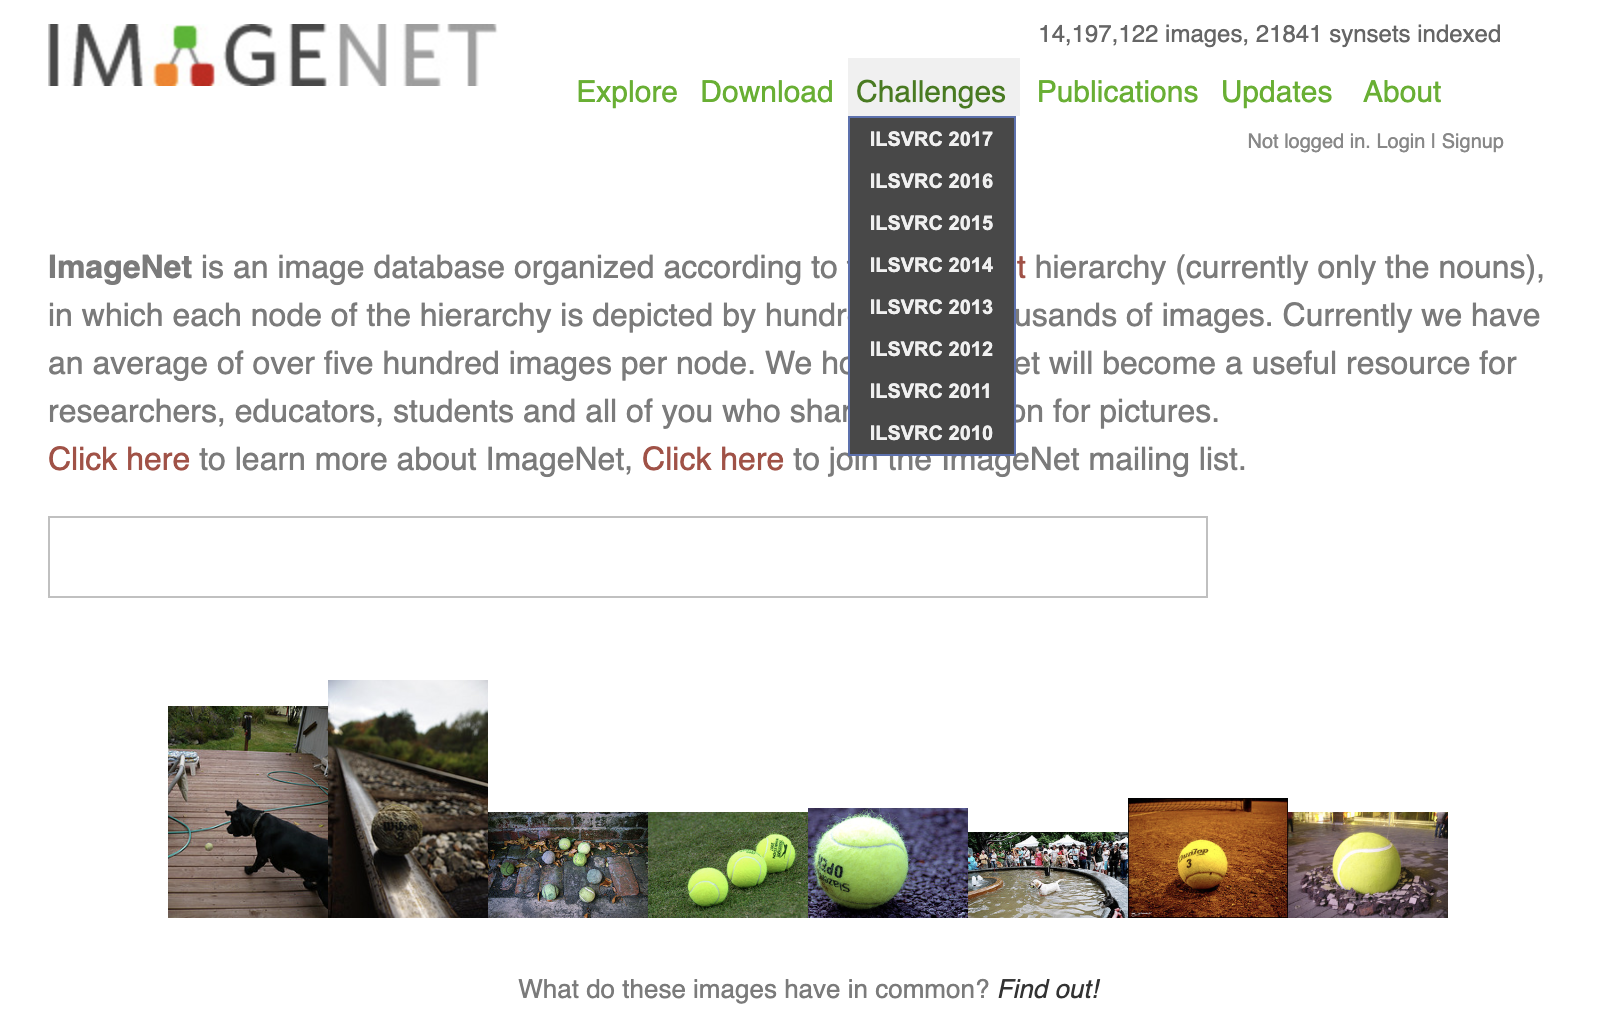
\includegraphics[width=.8\textwidth]{imagenet_page.png}
	\end{center}
\end{frame}

\begin{frame}
	\frametitle{modern neural networks}
	\small
	All changed with the introduction of AlexNet and the 2012 ImageNet Challenge...
	\begin{center}
		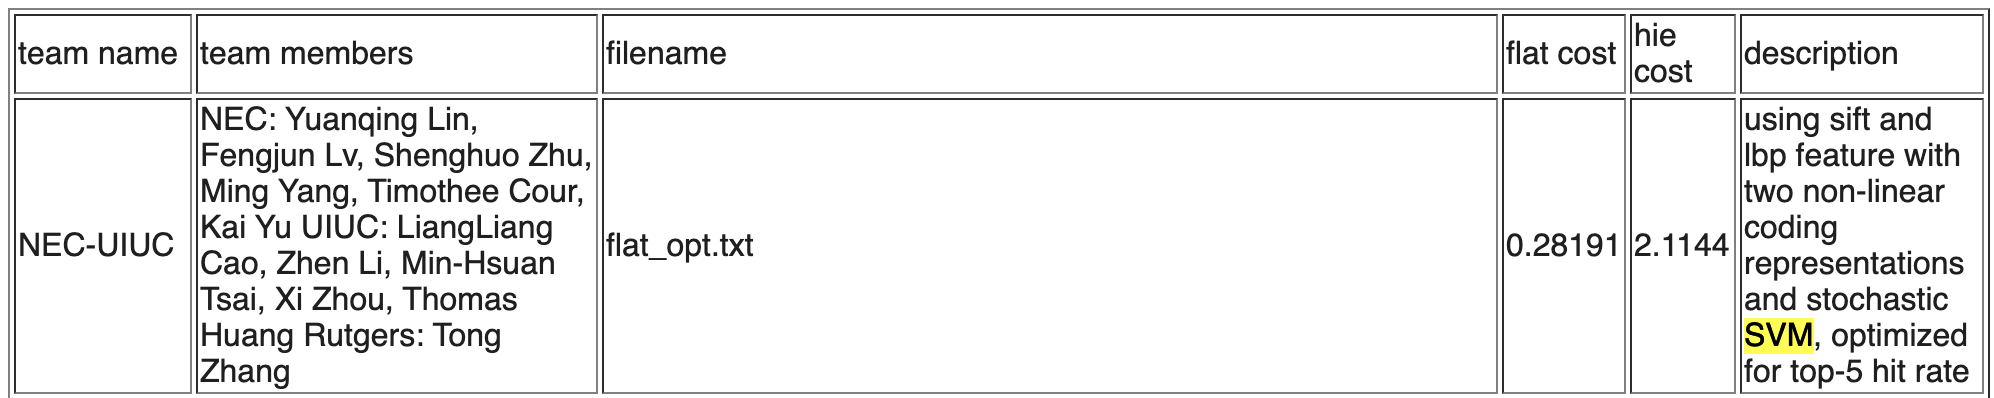
\includegraphics[width=.7\textwidth]{imagenet2010.png}
		
		2010 Results
	\end{center}
	\begin{center}
	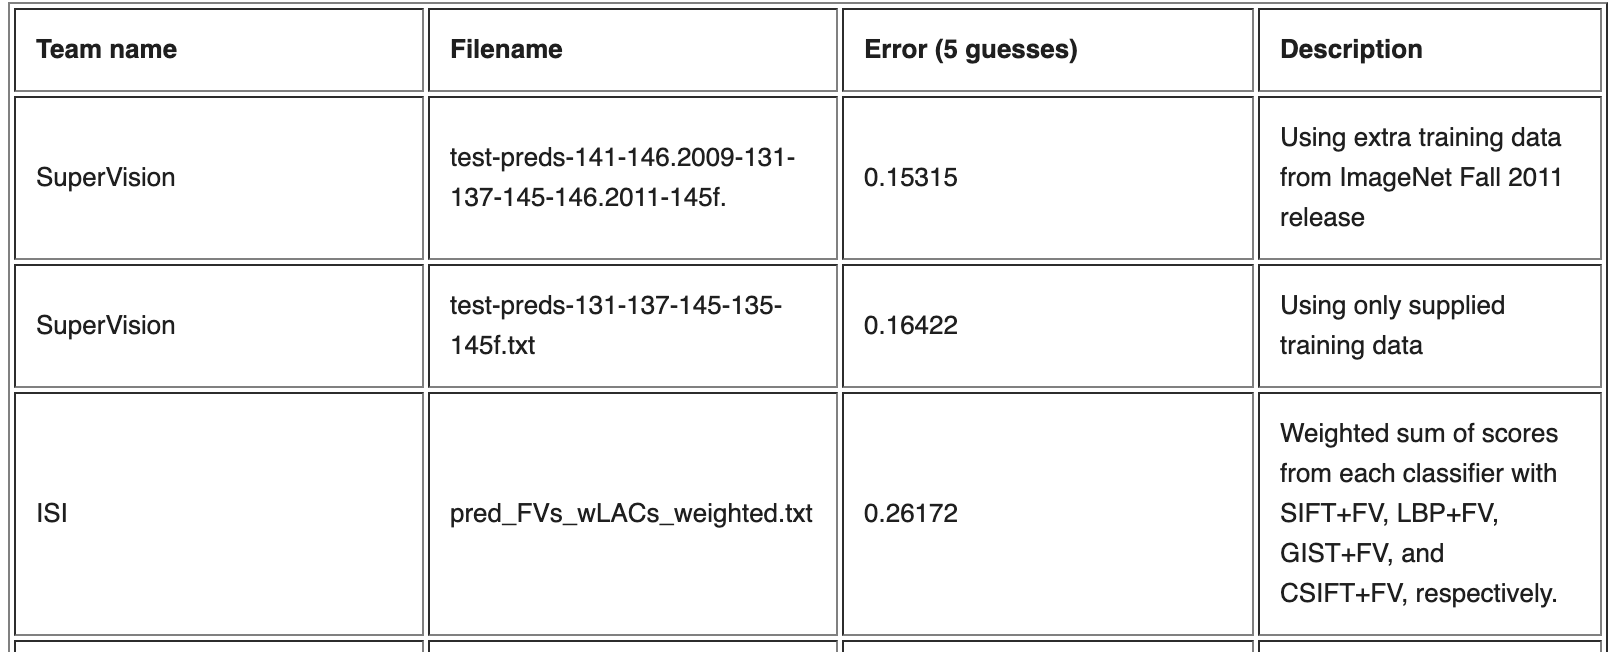
\includegraphics[width=.7\textwidth]{imagenet2012.png}
	
	2012 Results
	\end{center}
\end{frame}

\begin{frame}
	\frametitle{modern neural networks}
	\textbf{Why 2012?}
	\begin{itemize}
		\item Clever ideas in changing neural network architectures. 
		\item Wide-spread access to GPU computing power (CUDA and publicly available Nvidia GPU first released in 2007).
	\end{itemize}
\end{frame}

\begin{frame}
	\frametitle{2019 turing award winners}
	\small
``For conceptual and engineering breakthroughs that have made deep neural networks a critical component of computing.''
		\begin{center}
		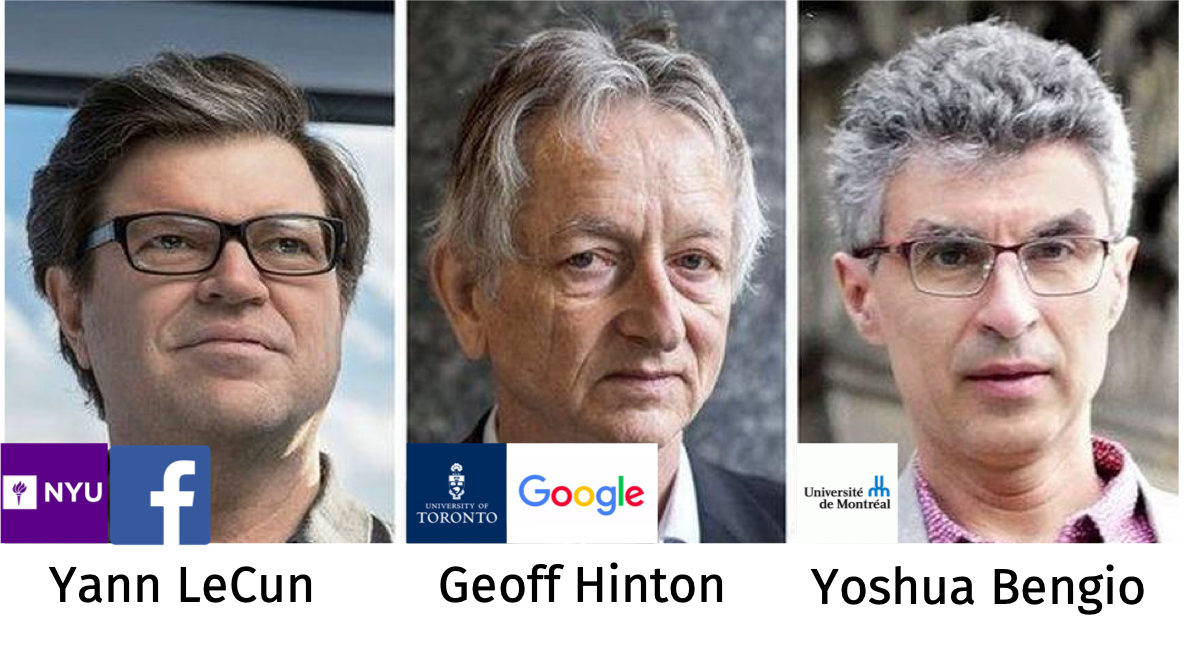
\includegraphics[width=.7\textwidth]{turing_annotate.png}
	\end{center}
\end{frame}

\begin{frame}
	\frametitle{use outside of computer science}
	\small
	Neural networks are flexible and relatively easy to understand conceptually, so they are also having impact in application areas outside of computer science. 
		\begin{center}
		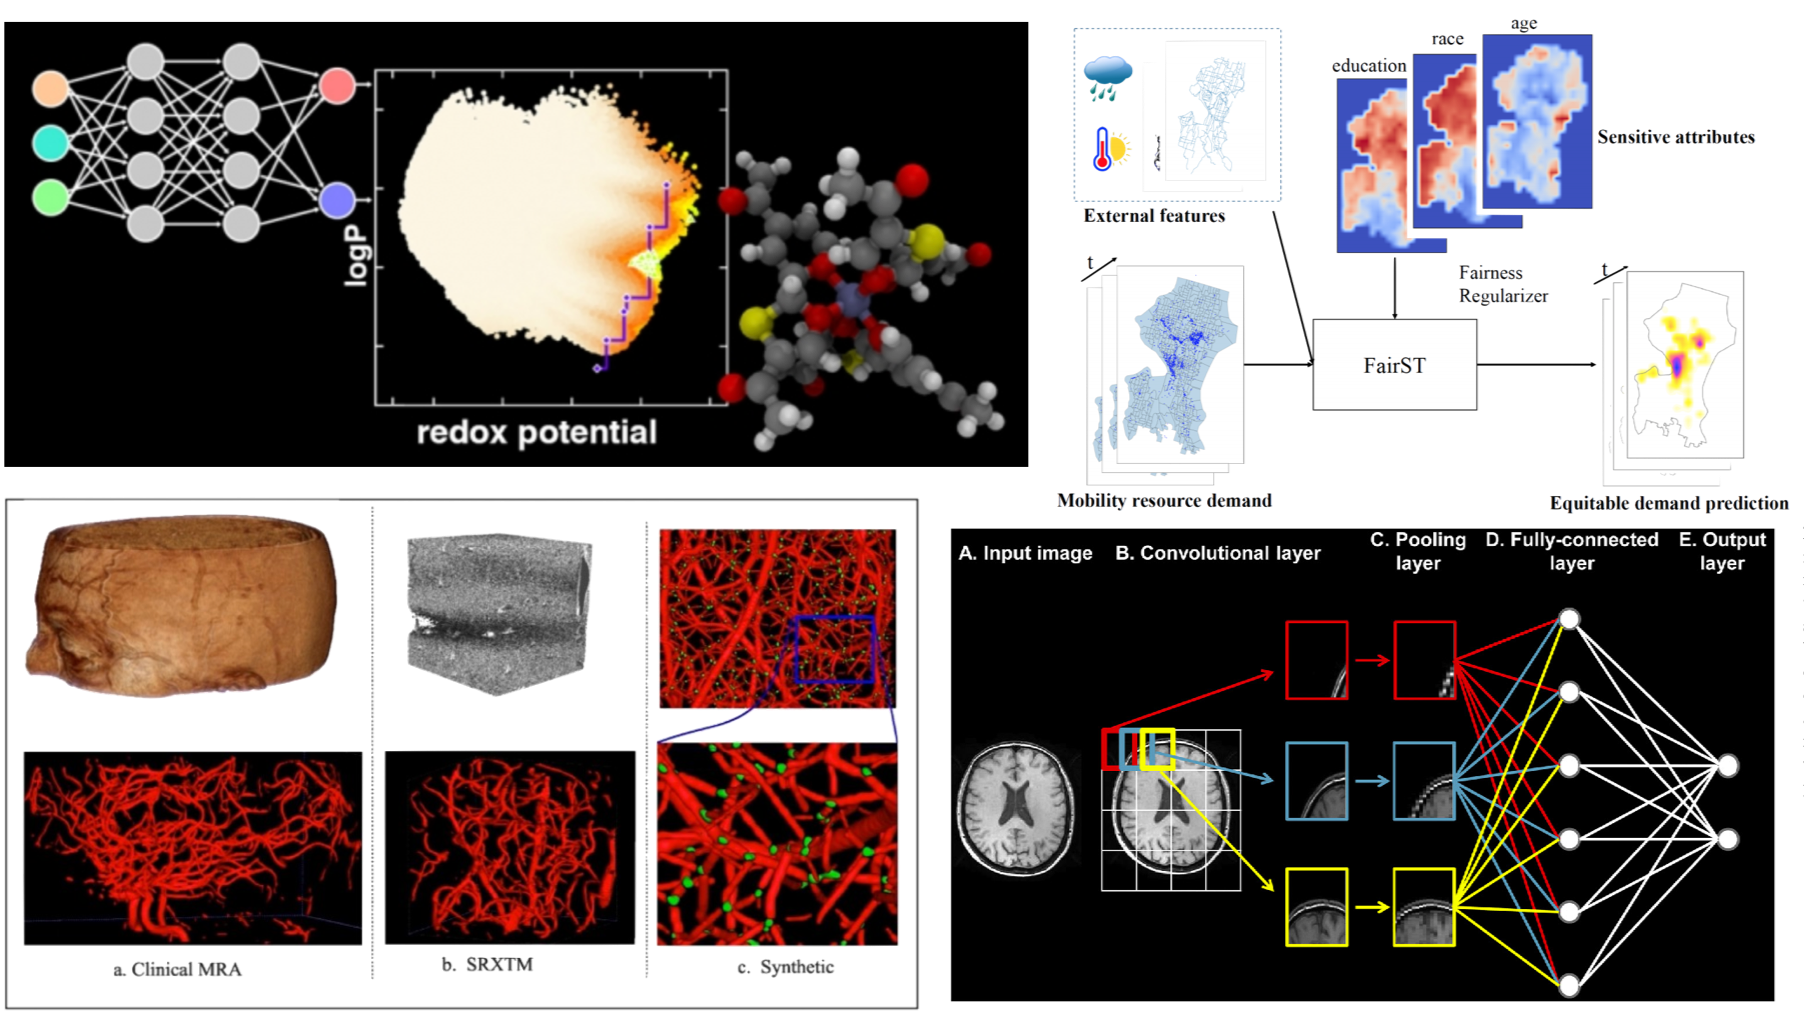
\includegraphics[width=.7\textwidth]{science_apps.png}
	\end{center}
	
 	Researchers working in the medicine, natural sciences, engineering, etc. are having a lot of luck implementing and applying these models to their data problems.
\end{frame}

\end{document} 






